%\documentclass[12pt]{article}
 %\documentclass[letterpaper,floatfix,citeautoscript,aip,jcp]{revtex4-1}
 %\documentclass[letterpaper,floatfix,citeautoscript,showkeys]{revtex4-1}
 %\documentclass[twocolumn,letterpaper,floatfix,citeautoscript,jcp]{revtex4-1}
 %\documentclass[twocolumn,letterpaper,floatfix,citeautoscript,aip,jcp]{revtex4-1}
 \documentclass[journal=jced,manuscript=article]{achemso}
 \setkeys{acs}{maxauthors=30,etalmode=truncate,articletitle=true}
 %%%%%%%%%%%%%%%%%%%%%%%%%%%%%%%%%%%%%%%%%%%%%%%%%%%%%%%%%%%%%%%%%%%%%
 %% Place any additional packages needed here.  Only include packages
 %% which are essential, to avoid problems later.
 %%%%%%%%%%%%%%%%%%%%%%%%%%%%%%%%%%%%%%%%%%%%%%%%%%%%%%%%%%%%%%%%%%%%%
 \usepackage{chemformula} % Formula subscripts using \ch{}
 \usepackage[T1]{fontenc} % Use modern font encodings
 
 %%%%%%%%%%%%%%%%%%%%%%%%%%%%%%%%%%%%%%%%%%%%%%%%%%%%%%%%%%%%%%%%%%%%%
 %% If issues arise when submitting your manuscript, you may want to
 %% un-comment the next line.  This provides information on the
 %% version of every file you have used.
 %%%%%%%%%%%%%%%%%%%%%%%%%%%%%%%%%%%%%%%%%%%%%%%%%%%%%%%%%%%%%%%%%%%%%
 %%\listfiles
 
 %%%%%%%%%%%%%%%%%%%%%%%%%%%%%%%%%%%%%%%%%%%%%%%%%%%%%%%%%%%%%%%%%%%%%
 %% Place any additional macros here.  Please use \newcommand* where
 %% possible, and avoid layout-changing macros (which are not used
 %% when typesetting).
 %%%%%%%%%%%%%%%%%%%%%%%%%%%%%%%%%%%%%%%%%%%%%%%%%%%%%%%%%%%%%%%%%%%%%
% \newcommand*\mycommand[1]{\texttt{\emph{#1}}}

\usepackage{fullpage}
\usepackage{amsfonts}
\usepackage{graphicx}
\usepackage{float}
\usepackage{amsmath}
\usepackage{chemfig}
\usepackage{indentfirst}
\usepackage{longtable}
\usepackage{array}
\usepackage{cellspace}
\usepackage{palatino}
%\usepackage{breqn}
\usepackage{amssymb}
\usepackage{verbatim}
\usepackage[hidelinks,colorlinks=false,citecolor=black,linkcolor=black]{hyperref}
\usepackage{siunitx}
\usepackage{xr}

\makeatletter
\newcommand*{\addFileDependency}[1]{% argument=file name and extension
	\typeout{(#1)}
	\@addtofilelist{#1}
	\IfFileExists{#1}{}{\typeout{No file #1.}}
}
\makeatother

\newcommand*{\myexternaldocument}[1]{%
	\externaldocument{#1}%
	\addFileDependency{#1.tex}%
	\addFileDependency{#1.aux}%
}

\myexternaldocument{JCED_FOMMS_supporting_information}

\SectionNumbersOn

% The figures are in a figures/ subdirectory.
\graphicspath{{figures/}}

%\bibliographystyle{apsrevlong}
%\bibliographystyle{apsrev}
\bibliographystyle{unsrt}

% italicized boldface for math (e.g. vectors)
\newcommand{\bfv}[1]{{\mbox{\boldmath{$#1$}}}}
% non-italicized boldface for math (e.g. matrices)
\newcommand{\bfm}[1]{{\bf #1}}          

%\newcommand{\bfm}[1]{{\mbox{\boldmath{$#1$}}}}
%\newcommand{\bfm}[1]{{\bf #1}}
\newcommand{\expect}[1]{\left \langle #1 \right \rangle} % <.> for denoting expectations over realizations of an experiment or thermal averages

\newcommand{\var}[1]{{\mathrm var}{(#1)}}
\newcommand{\x}{\bfv{x}}
\newcommand{\y}{\bfv{y}}
\newcommand{\f}{\bfv{f}}

\newcommand{\hatf}{\hat{f}}

\newcommand{\bTheta}{\bfm{\Theta}}
\newcommand{\btheta}{\bfm{\theta}}
\newcommand{\bhatf}{\bfm{\hat{f}}}
\newcommand{\Cov}[1] {\mathrm{cov}\left( #1 \right)}
\newcommand{\T}{\mathrm{T}}                                % T used in matrix transpose

\newcommand\blfootnote[1]{%
	\begingroup
	\renewcommand\thefootnote{}\footnote{#1}%
	\addtocounter{footnote}{-1}%
	\endgroup
}

\author{Richard A. Messerly}
\email{richard.messerly@nist.gov}
\affiliation{Thermodynamics Research Center, National Institute of Standards and Technology, Boulder, Colorado, 80305, United States}

\author{Mohammad S. Barhaghi}
\affiliation{Department of Chemical Engineering and Materials Science, Wayne State University, Detroit, Michigan 48202, United States}

\author{Jeffrey J. Potoff}
\affiliation{Department of Chemical Engineering and Materials Science, Wayne State University, Detroit, Michigan 48202, United States}

\author{Michael R. Shirts}
\affiliation{Department of Chemical and Biological Engineering, University of Colorado, Boulder, Colorado, 80309, United States}

%%%%%%%%%%%%%%%%%%%%%%%%%%%%%%%%%%%%%%%%%%%%%%%%%%%%%%%%%%%%%%%%%%%%%
%% The document title should be given as usual. Some journals require
%% a running title from the author: this should be supplied as an
%% optional argument to \title.
%%%%%%%%%%%%%%%%%%%%%%%%%%%%%%%%%%%%%%%%%%%%%%%%%%%%%%%%%%%%%%%%%%%%%
%\title{Multistate Bennett Acceptance Ratio replaces histogram reweighting for vapor-liquid coexistence calculations}
%\title{Multistate Bennett Acceptance Ratio to enable rapid force field parameterization}
%\title{Multistate Bennett Acceptance Ratio as a substitute for histogram reweighting when optimizing non-bonded parameters}
%\title{Multistate reweighting provides a better alternative to histogram reweighting for coexistance calculations}
%\title{Multistate histogram-free reweighting for vapor-liquid coexistence calculations of non-simulated force field parameters}
%\title{Estimating vapor-liquid coexistence properties with histogram-free reweighting}
%\title{Histogram-free reweighting for vapor-liquid coexistence calculations of multiple force fields}
\title{Histogram-free reweighting to estimate vapor-liquid coexistence properties of non-simulated force fields}

%%%%%%%%%%%%%%%%%%%%%%%%%%%%%%%%%%%%%%%%%%%%%%%%%%%%%%%%%%%%%%%%%%%%%
%% Some journals require a list of abbreviations or keywords to be
%% supplied. These should be set up here, and will be printed after
%% the title and author information, if needed.
%%%%%%%%%%%%%%%%%%%%%%%%%%%%%%%%%%%%%%%%%%%%%%%%%%%%%%%%%%%%%%%%%%%%%
%\abbreviations{IR,NMR,UV}
\keywords{MBAR, Monte Carlo, Grand Canonical, Vapor-liquid equilibria}

%%%%%%%%%%%%%%%%%%%%%%%%%%%%%%%%%%%%%%%%%%%%%%%%%%%%%%%%%%%%%%%%%%%%%
%% The manuscript does not need to include \maketitle, which is
%% executed automatically.
%%%%%%%%%%%%%%%%%%%%%%%%%%%%%%%%%%%%%%%%%%%%%%%%%%%%%%%%%%%%%%%%%%%%%
\begin{document}
	
	%%%%%%%%%%%%%%%%%%%%%%%%%%%%%%%%%%%%%%%%%%%%%%%%%%%%%%%%%%%%%%%%%%%%%
	%% The "tocentry" environment can be used to create an entry for the
	%% graphical table of contents. It is given here as some journals
	%% require that it is printed as part of the abstract page. It will
	%% be automatically moved as appropriate.
	%%%%%%%%%%%%%%%%%%%%%%%%%%%%%%%%%%%%%%%%%%%%%%%%%%%%%%%%%%%%%%%%%%%%%
%	\begin{tocentry}
%	\end{tocentry}

%\blfootnote{Contribution of NIST, an agency of the United States government; not subject to copyright in the United States.}

\section*{Abstract}

The prediction of accurate vapor-liquid coexistence properties with molecular simulation relies on well-parameterized force fields. Histogram reweighting (HR) is a standard approach for converting Grand Canonical Monte Carlo (GCMC) simulation output into vapor-liquid coexistence properties (saturated liquid density, $\rho_{\rm liq}^{\rm sat}$, saturated vapor density, $\rho_{\rm vap}^{\rm sat}$, saturated vapor pressures, $P_{\rm vap}^{\rm sat}$, and enthalpy of vaporization, $\Delta H_{\rm v}$). Due to the abundance of experimental vapor-liquid coexistence data and the sensitivity of such properties to both short- and long-range non-bonded interactions, numerous force fields have been parameterized using $\rho_{\rm liq}^{\rm sat}$, $\rho_{\rm vap}^{\rm sat}$, $P_{\rm vap}^{\rm sat}$, and/or $\Delta H_{\rm v}$. Unfortunately, computing $\rho_{\rm liq}^{\rm sat}$, $\rho_{\rm vap}^{\rm sat}$, $P_{\rm vap}^{\rm sat}$, and/or $\Delta H_{\rm v}$ for each proposed parameter set requires a large amount of GCMC simulations. 
	
We demonstrate how a histogram-free reweighting approach can alleviate the computational burden of force field parameterization. Specifically, we utilize the Multistate Bennett Acceptance Ratio (MBAR) to estimate coexistence properties for non-bonded parameters without simulating each parameter set directly. Thus, MBAR greatly reduces the amount of GCMC simulations that are required for parameterizing the non-bonded potential.

First, we validate that GCMC-MBAR and GCMC-HR yield indistinguishable results when computing coexistence properties for only the simulated force field. Second, we utilize GCMC-MBAR to optimize compound-specific parameters, where simulations are only performed with the initial ``transferable'' parameter set. Third, we predict coexistence properties of force field $j$ by simulating force field $i$, where $i$ and $j$ are common force fields from the literature. Fourth, we simulate cyclohexane with a common united-atom Lennard-Jones 12-6 potential (Transferable Potentials for Phase Equilibria, TraPPE) to predict coexistence properties over a wide range of Mie $\lambda$-6 (generalized Lennard-Jones) parameters ($\epsilon$, $\sigma$, and $\lambda$). We provide guidelines for determining the accuracy of GCMC-MBAR predicted $\rho_{\rm liq}^{\rm sat}$, $\rho_{\rm vap}^{\rm sat}$, $P_{\rm vap}^{\rm sat}$, and/or $\Delta H_{\rm v}$ values for non-simulated force fields. 

% potentials for cyclohexane. where only the Lennard-Jones parameters are simulated directly. % without performing any additional simulations.

\section{Introduction}

A key use of molecular simulation is the ability to accurately and efficiently estimate vapor-liquid coexistence properties, i.e., saturated liquid density $(\rho_{\rm liq}^{\rm sat})$, saturated vapor density $(\rho_{\rm vap}^{\rm sat})$, saturated vapor pressures $(P_{\rm vap}^{\rm sat})$, and enthalpy of vaporization $(\Delta H_{\rm v})$. The accuracy of coexistence estimates depends on the underlying molecular model (a.k.a., force field, potential model, or Hamiltonian) while the computational efficiency depends primarily on the simulation methods, software, and hardware.

Several simulation approaches exist for computing vapor-liquid coexistence properties \cite{Pana2000}. These include Gibbs Ensemble Monte Carlo (GEMC), two-phase molecular dynamics (2$\phi$MD) \cite{Fern2007}, isothermal-isochoric integration (ITIC) \cite{Mostafa2018}, and Grand Canonical Monte Carlo coupled with histogram reweighting (GCMC-HR). The improved efficiency of these methods has greatly enabled the development of accurate force fields \cite{TraPPE,TAMie,Mie,AUA4,Mess4}. However, parameterization of non-bonded interactions with vapor-liquid coexistence calculations over a wide range of temperatures remains an arduous and time-consuming task.

%Due to the abundance of experimental vapor-liquid coexistence data and the sensitivity of such properties to both short- and long-range non-bonded interactions, numerous force fields \cite{TraPPE,Mie,TAMie,AUA4,Mess4} have been parameterized using $\rho_{\rm liq}^{\rm sat}$, $\rho_{\rm vap}^{\rm sat}$, $P_{\rm vap}^{\rm sat}$, and/or $\Delta H_{\rm v}$. Although the development of accurate force fields has been greatly enabled by the improved efficiency of simulation methods, parameterization of non-bonded interactions with vapor-liquid coexistence calculations remains an arduous and time-consuming task \cite{TraPPE,TAMie,Mie}.

% Advantages and disadvantages exist for each method. For example, GEMC and GCMC require insertion moves that are computationally inefficient for complex molecular structures with high density liquid phases. Several advanced simulation techniques are available to overcome this challenge \cite{ConBias}, which has enabled GEMC and GCMC-HR to be the primary methods of choice for vapor-liquid coexistence calculations.

%Some clear advantages and disadvantages exist for GCMC-HR compared with GEMC. For example, one advantage of GCMC-HR is the higher precision \cite{GEMC_GCMC}. Furthermore, coexistence properties can be computed at temperatures that are not simulated directly. However, GEMC is arguably more straightforward in that simulations are performed only at the desired saturation temperatures $(T^{\rm sat})$. By contrast, GCMC-HR requires a series of GCMC simulations for a single $T^{\rm sat}$. This set includes a near-critical simulation that ``bridges'' the vapor and liquid phases. Obtaining the appropriate chemical potential $(\mu)$ for this bridge simulation is a cumbersome and, typically, iterative process (although more advanced methods exist to obtain a good initial estimate for $\mu$ \cite{Hemmen2015}).

%Another disadvantage of GCMC-HR compared to GEMC is that GCMC-HR requires more post-processing (i.e., histogram reweighting), while simple block averaging is typically sufficient for GEMC. 

%Histogram reweighting (and more generally, configuration reweighting) is an important tool in many fields of molecular simulation. In fact, it has long since been known that it is possible to estimate properties for state $j$ by reweighting configurations that were sampled with state $i$. \cite{McDonald1967,Card1970,Wood1968,Pana2000} For example, umbrella sampling simulations are often processed using the weighted histogram analysis method (WHAM) to compute free energy differences between states. A popular alternative to WHAM is the Multistate Bennett Acceptance Ratio (MBAR) \cite{chodera:jctc:2007,shirts-chodera:jcp:2008:mbar}, which is readily available in the \textit{pymbar} package.

Our primary objective is to reduce the computational cost of optimizing non-bonded parameters with vapor-liquid saturation properties. This is achieved by substituting histogram reweighting with the Multistate Bennett Acceptance Ratio (MBAR), \cite{chodera:jctc:2007,shirts-chodera:jcp:2008:mbar} a histogram-free reweighting schema. The proposed GCMC-MBAR method is identical to the traditional GCMC-HR approach except that it uses MBAR to reweight configurations rather than reweighting histograms. The benefit of this simple modification is that GCMC-MBAR can estimate coexistence properties for non-bonded parameter sets that have not been simulated directly. 

% we perform GCMC simulations and reweight the configurations with MBAR to predict vapor-liquid coexistence properties for non-bonded parameter sets that are not simulated directly.  substitute traditional HR with MBAR to obtain a GCMC-MBAR method for computing vapor-liquid coexistence properties. Because MBAR reweights configurations rather than histograms, GCMC-MBAR can estimate coexistence properties for non-bonded parameter sets that have not been simulated directly. 
%
%MBAR is a histogram-free reweighting approach, that we use in place of the standard HR  which is substituted for HR in the standard GCMC-HR approach.
%
%In this study, we substitute HR with MBAR for the GCMC-HR approach of computing vapor-liquid coexistence properties. Section \ref{sec: GCMC-HR and GCMC-MBAR} demonstrates that MBAR and HR are mathematically equivalent (in the limit of zero bin width) while Section \ref{sec: Results} shows that they are also numerically equivalent (to within statistical uncertainties). Boulougouris et al. demonstrate how to combine HR with GEMC (GEMC-HR) to estimate saturation properties at non-simulated temperatures \cite{Boulougouris2010}, therefore, MBAR could alternatively be applied to GEMC simulations.

%this study presents how MBAR can be used with GCMC simulations
%
%  HR is more commonly applied to GCMC than GEMC simulations (for an example of GEMC-HR see Ref. \citenum{Boulougouris2010}) is not unique to GCMC simulations (see Ref. \citenum{Boulougouris2010} where HR is applied to GEMC-HR) As histogram reweighting is already an essential tool for GCMC-HR, we substitute HR with MBAR  in the GCMC-HR approach of computing vapor-liquid coexistence properties. Section \ref{sec: GCMC-HR and GCMC-MBAR} demonstrates that MBAR and HR are mathematically equivalent (in the limit of zero bin width) while Section \ref{sec: Results} shows that they are also numerically equivalent (to within statistical uncertainties). Boulougouris et al. demonstrate how to combine HR with GEMC (GEMC-HR) to estimate saturation properties at non-simulated temperatures \cite{Boulougouris2010}, therefore, MBAR could alternatively be applied to GEMC simulations.

%Similar to the HR MBAR could alternatively be applied to GEMC simulations in an approach similar to the histogram reweighting GEMC  that of Boulougouris et al. demonstrate how to combine HR with GEMC (GEMC-HR) to estimate saturation properties at non-simulated temperatures \cite{Boulougouris2010}, therefore, MBAR could alternatively be applied to GEMC simulations.

%Histogram reweighting (and more generally, configuration reweighting) is an important tool in many fields of molecular simulation. In fact, it has long since been known that it is possible to estimate properties for state $j$ by reweighting configurations that were sampled with state $i$. \cite{McDonald1967,Card1970,Wood1968,Pana2000} For example, umbrella sampling simulations are often processed using the weighted histogram analysis method (WHAM) to compute free energy differences between states. A popular alternative to WHAM is the Multistate Bennett Acceptance Ratio (MBAR) \cite{chodera:jctc:2007,shirts-chodera:jcp:2008:mbar}, which is readily available in the \textit{pymbar} package.

In similar studies, Messerly et al. demonstrate how to combine MBAR with ITIC (MBAR-ITIC) to optimize generalized Lennard-Jones (Mie $\lambda$-6) potentials \cite{Postdoc_1,Postdoc_2}. For MBAR-ITIC, a series of constant number of molecules, constant volume, and constant temperature $(NVT)$ simulations are performed along an isotherm and isochore(s) with a ``reference'' force field(s) $(\theta_{\rm ref})$. MBAR reweights configurations sampled with $\theta_{\rm ref}$ to estimate the internal energy $(U)$ and pressure $(P)$ at each $(T$, $\rho)$ state point for a non-simulated (``rerun'') force field $(\theta_{\rm rr})$. ITIC then converts the $U$ and $P$ estimates into vapor-liquid coexistence properties \cite{Mostafa_Diss,Mostafa2018}.

%In this study, we substitute HR with MBAR for the GCMC-HR approach of computing vapor-liquid coexistence properties. Section \ref{sec: GCMC-HR and GCMC-MBAR} demonstrates that MBAR and HR are mathematically equivalent (in the limit of zero bin width) while Section \ref{sec: Results} shows that they are also numerically equivalent (to within statistical uncertainties). Boulougouris et al. demonstrate how to combine HR with GEMC (GEMC-HR) to estimate saturation properties at non-simulated temperatures \cite{Boulougouris2010}, therefore, MBAR could alternatively be applied to GEMC simulations.

%and example scripts are included as Supporting Information to promote future implementation.  

%In this study, we utilize an alternative to histogram reweighting, namely, the Multistate Bennett Acceptance Ratio (MBAR) . MBAR is readily available in the \textit{pymbar} package and example scripts are included as Supporting Information to promote future implementation. Section \ref{sec: GCMC-HR and GCMC-MBAR} demonstrates that MBAR and HR are mathematically equivalent (in the limit of zero bin width) while Section \ref{sec: Results} shows that they are also numerically equivalent (to within statistical uncertainties). Note that Boulougouris et al. combine HR with GEMC (GEMC-HR) to estimate saturation properties at non-simulated temperatures \cite{Boulougouris2010}. Therefore, although we apply MBAR to GCMC simulations, the approach can also be applied to GEMC simulations.

%In this study, we utilize the Multistate Bennett Acceptance Ratio (MBAR) Grand Canonical Monte Carlo (GCMC-MBAR) as a substitute for GCMC-HR. We demonstrate that MBAR and HR are mathematically equivalent (in the limit of zero bin width) as well as practically equivalent (to within statistical uncertainties). Note that Boulougouris et al. demonstrate how HR can be applied to GEMC output (GEMC-HR) to estimate saturation properties at non-simulated temperatures \cite{Boulougouris2010}. Therefore, although we apply MBAR to GCMC simulations, the approach can also be applied to GEMC simulations.
%
%
%
%Although GEMC appears to be slightly more popular amongst simulation practitioners, this study utilizes the GCMC approach. GCMC-HR has been shown to

%In this study we demonstrate how the Multistate Bennett Acceptance Ratio is mathematically equivalent to histogram reweighting 
%%% Old version
%Although GCMC-HR has a higher precision than GEMC, GEMC remains a more popular method amongst simulation practitioners. There are at least two potential reasons why GEMC has grown in popularity relative to GCMC-HR. First, GEMC is more straightforward in that, GEMC simulations are performed directly at the desired saturation temperature $(T^{\rm sat})$. By contrast, GCMC-HR requires a series of GCMC simulations for a single $T^{\rm sat}$ (although this is also an advantage of GCMC-HR as estimates can be obtained at any $T^{\rm sat}$ value without additional simulations). This set includes a near-critical simulation that ``bridges'' the vapor and liquid phases. Obtaining an initial guess for the chemical potential $(\mu)$ of this bridge simulation is a cumbersome and, typically, iterative process, although more advanced methods do exist to obtain a good initial estimate for $\mu$ (e.g., Hemmen et al. \cite{Hemmen2015}). 
%
%A likely second reason for increased popularity of GEMC is that GCMC-HR requires a great deal of post-processing (i.e., histogram reweighting), while simple block averaging is typically sufficient for GEMC. In this study, we introduce an alternative to histogram reweighting, namely, the Multistate Bennett Acceptance Ratio (MBAR) \cite{chodera:jctc:2007,shirts-chodera:jcp:2008:mbar}. MBAR is readily available in the \textit{pymbar} package and example scripts are included as Supporting Information to promote future implementation.
%
%Histogram reweighting (and more generally, configuration reweighting) is an important tool in many fields of molecular simulation. In fact, it has long since been known that it is possible to estimate properties for state ``j'' by reweighting configurations that were sampled with state ``i.'' \cite{McDonald1967,Card1970,Wood1968,Pana2000} For example, umbrella sampling simulations are often processed using the weighted histogram analysis method (WHAM) to compute free energy differences between states. In addition, Boulougouris et al. demonstrated how histogram reweighting can be applied to GEMC output to estimate saturation properties at non-simulated temperatures (analogous to GCMC-HR) \cite{Boulougouris2010}.
%
%Although the development of accurate force fields has been greatly enabled by the efficiency of the aforementioned simulation methods (e.g., GEMC, GCMC-HR), parameterization of non-bonded interactions with vapor-liquid coexistence calculations remains an arduous and time-consuming task \cite{TraPPE,TAMie,Mie}. MBAR-GCMC not overly serves as a substitute for MBAR-HR, but MBAR can also be used to estimate properties for non-simulated parameter sets. For example, recently, Messerly et al. demonstrated how MBAR coupled with ITIC (MBAR-ITIC) enables rapid force field parameterization by estimating coexistence properties for non-simulated parameter sets \cite{Postdoc_1,Postdoc_2}. 

%
%Although histogram reweighting requires additional analysis steps, the benefits of histogram reweighting are clear. For example

%Although histogram reweighting approaches are common in some fields of molecular simulation, e.g., WHAM is commonly used for computing free energies, most open-source Monte Carlo codes do not include a HR tool and, thus, in-house post-processing codes abound. In this study, we introduce an alternative to histogram reweighting, namely, the Multistate Bennett Acceptance Ratio (MBAR). MBAR is readily available in the \textit{pymbar} package and example scripts are included as Supporting Information to promote future implementation.

%, with a near-critical simulation that ``bridges'' the vapor and liquid phases.

%For example, the exponential-6 model of Errington and Panagiotoupoulos
%The method outlined in this study is similar in spirit to the ``Hamiltonian scaling'' (HS) approach utilized with GEMC (BLANK) and GCMC-HR (BLANK).

%A closely related method to histogram reweighting, and one that is similar in spirit to the method outlined in the present study, is ``Hamiltonian scaling'' (HS). Despite Hamiltonian scaling Grand Canonical Monte Carlo (HS-GCMC) proving to be a powerful tool to obtain coexistence curves for multiple force fields from a single set of simulations, it has yet to gain widespread popularity. This is likely due to the added complexity of the algorithm, where the prescribed $\mu$ and $T$ change during the coarse of the GCMC simulation, depending on which Hamiltonian (force field) is being sampled. Furthermore, the post-processing requires a slightly more complicated form of histogram reweighting. Also, HS requires a decision be made \textit{a priori} regarding which Hamiltonians are to be tested. By contrast, MBAR does not require any modification of the simulation procedure, the post-processing is essentially unchanged, and the Hamiltonians need not be selected prior to the simulations.
 
%Substituting the standard HR approach with MBAR is not the primary purpose of this study. Rather, we demonstrate how GCMC-MBAR can also estimate coexistence properties for non-simulated parameter sets, which can greatly accelerate force field parameterization. In a similar study, Messerly et al. demonstrate how to combine MBAR with ITIC (MBAR-ITIC) to optimize Mie $\lambda$-6 (generalized Lennard-Jones) potentials \cite{Postdoc_1,Postdoc_2}. For MBAR-ITIC, a series of $NVT$ simulations along an isotherm and isochores are performed with a ``reference'' force field $(\theta_{\rm ref})$. MBAR computes the internal energy $(U)$ and pressure $(P)$ (or compressibility factor, $Z$) for each $T-\rho$ state point with a non-simulated (``rerun'') force field $(\theta_{\rm rr})$. ITIC then converts the $U$ and $P$ values into vapor-liquid coexistence properties \cite{Mostafa_Diss,Mostafa2018}.

%, where $U$ and $P$ are estimated by performing $NVT$ simulations and reweighting the configurations with MBAR.

% at numerous temperatures and densities, \cite{Mostafa_Diss,Mostafa2018} these values are estimated by performing $NVT$ simulations and reweighting the configurations with MBAR.

% for parameter sets near the ``reference'' parameter set from which configurations are sampled 

The results from Messerly et al. demonstrate that MBAR-ITIC is most reliable in the local domain, i.e., when $\theta_{\rm rr} \approx \theta_{\rm ref}$ \cite{Postdoc_1}. Furthermore, MBAR-ITIC performs best for changes in the non-bonded well-depth parameter $(\epsilon)$ while it performs significantly worse for large changes in the non-bonded size $(\sigma)$ and repulsive $(\lambda)$ parameters. This ``poor overlap'' when $\theta_{\rm rr} \not\approx \theta_{\rm ref}$ can be quantified by the number of effective snapshots $(K^{\rm eff}_{\rm snaps})$, which is essentially the number of non-negligible samples that contribute to the estimated ensemble averages. Poor overlap (low $K^{\rm eff}_{\rm snaps}$) is especially problematic for MBAR-ITIC as a large number of snapshots is needed to obtain precise estimates of $P$ in the liquid phase, due to large fluctuations in $P$ at high densities.

% which are essential to obtain reasonable values of $\rho_{\rm liq}^{\rm sat}$.

%MBAR not only serves as a substitute for histogram reweighting in the standard GCMC-HR approach, but GCMC-MBAR can also be used to estimate coexistence properties for non-simulated parameter sets, which can greatly accelerate force field parameterization. In a similar study, Messerly et al. demonstrate how to combine MBAR with ITIC (MBAR-ITIC) to optimize Mie $\lambda$-6 (generalized Lennard-Jones) potentials \cite{Postdoc_1,Postdoc_2}. Since ITIC requires the internal energy $(U)$ and pressure $(P)$ (or compressibility factor, $Z$) at numerous temperatures and densities, \cite{Mostafa_Diss,Mostafa2018} these values are estimated by performing $NVT$ simulations and reweighting the configurations with MBAR. 

%The results from Messerly et al. demonstrate that MBAR-ITIC is most reliable in the local domain, i.e., for parameter sets near the ``reference'' parameter set from which configurations are sampled \cite{Postdoc_1}. Furthermore, MBAR-ITIC performs best for changes in the non-bonded well-depth parameter $(\epsilon)$ while it performs significantly worse for large changes in the non-bonded size and repulsive parameters $(\sigma$ and $\lambda$, respectively$)$. This is typically referred to as poor ``overlap.''

%precise $P$ calculations in the supercritical and liquid phase, which necessitates

Our initial hypothesis was that GCMC-MBAR would experience better overlap than was observed for MBAR-ITIC when $\theta_{\rm rr} \not\approx \theta_{\rm ref}$. There were two main reasons for this hypothesis/aspiration. First, as opposed to the fixed density $NVT$ simulations used in ITIC, the fluctuating density in GCMC simulations samples from a wider range of configurations and energies. Second, ITIC requires larger box sizes (and, thereby, more molecules) than those typically utilized with GCMC. By utilizing fewer molecules, GCMC simulations experience larger energy fluctuations (on a percent basis) which improves the overlap between states. We also hypothesized that the impact of poor overlap would be less severe compared to MBAR-ITIC, where poor overlap leads to sporadic values of $P$ and nonsensical coexistence estimates.  

%  require a large number of snapshots ITIC requires precise estimates of $P$ in the liquid phase, which necessitates a large number of of snapshots for

%configurations. $(NVT)$ does not sample from a wide range of energies  leads to large energy differences for small changes in $\sigma$ and $\lambda$. The fluctuating densities of GCMC simulations should accommodate greater changes in short-range interactions. 

The method outlined in this study is similar in spirit to ``Hamiltonian scaling'' (HS), which has been applied to both GEMC \cite{Kiyohara1996} and GCMC simulations \cite{Errington1998,Exp6,Errington1999,Pana2000}. The HS approach samples from multiple force fields (Hamiltonians) in a single simulation according to a weighted sampling probability. Vapor-liquid coexistence curves for each force field are estimated post-simulation by reweighting the configurations accordingly. For the GCMC implementation of Hamiltonian scaling (HS-GCMC), $\mu$ and $T$ are not stationary during the simulation, rather the current value of $\mu$ and $T$ depends on which force field is being sampled. Despite HS-GCMC proving to be a powerful tool to optimize force field parameters \cite{Errington1998,Exp6,Errington1999,Pana2000}, it has yet to gain widespread popularity. This is likely due to the added complexity of both the simulation protocol and the histogram post-processing. Also, HS requires that a decision be made \textit{a priori} regarding which force fields are to be tested. By contrast, GCMC-MBAR does not require any modification of the simulation procedure, the post-processing is essentially unchanged, and the non-bonded parameter sets need not be selected prior to the simulations.

%Recently, Weidler and Gross proposed ``individualized,'' i.e., compound-specific, parameter sets for compounds which contain large amounts of experimental data \cite{Weidler2018}. To avoid overfitting, a one-dimensional optimization is employed which scales $\epsilon$ for all united-atom sites while not adjusting $\sigma$ or $\lambda$. MBAR is ideally suited for this ``$\epsilon$-scaling'' approach for at least two reasons. First, as mentioned previously, MBAR is most reliable when extrapolating in $\epsilon$ rather than $\sigma$ and/or $\lambda$. Second, the rate-limiting step for MBAR is recomputing the configurational energies for a different force field. Furthermore, storing millions of configuration (``snapshots'') is highly memory intensive. While basis functions (see Section \ref{sec: Basis functions}) alleviate the additional computational cost and reduce the memory load, $\epsilon$-scaling does not require storing/recomputing configurations or basis functions. Instead, the energies for each snapshot are simply multiplied by the $\epsilon$-scaling parameter.  

%   Despite HS-GCMC proving to be a powerful tool to obtain coexistence curves for multiple force fields from a single set of simulations, it has yet to gain widespread popularity. This is likely due to the added complexity of the algorithm, where the prescribed $\mu$ and $T$ change during the coarse of the GCMC simulation, depending on which Hamiltonian (force field) is being sampled. Furthermore, the post-processing requires a slightly more complicated form of histogram reweighting. Also, HS requires a decision be made \textit{a priori} regarding which Hamiltonians are to be tested. By contrast, MBAR does not require any modification of the simulation procedure, the post-processing is essentially unchanged, and the Hamiltonians need not be selected prior to the simulations.

%The results from Messerly et al. demonstrated that MBAR is accurate over a wide range of $\epsilon$ (the Lennard-Jones well-depth parameter) values but less reliable for large changes in $\sigma$ (the Lennard-Jones size parameter) and $\lambda$ (the Mie $\lambda$-6 repulsive parameter, i.e., for Lennard-Jones 12-6 $\lambda = 12$). MBAR is most reliable in the local parameter space relative to the reference parameter set from which configurations are sampled.

%Some fundamental limitations exist for the MBAR-ITIC approach. First, ITIC is ill-suited for near-critical saturation properties, i.e., ITIC is not recommended for $T^{\rm sat} > 0.85 T_{\rm c}$ ($T_{\rm c}$ is the critical temperature). Second, ITIC requires a temperature correlation for the virial coefficients of the force field. Third, the poor extrapolation of MBAR with changes in $\sigma$ and $\lambda$.

The outline for this study is the following. Section \ref{sec: Methods} provides details regarding the force fields, simulation set-up, and the HR/MBAR post-simulation analysis. Section \ref{sec: Results} presents results of GCMC-MBAR for four scenarios in Sections \ref{sec: Constant theta} to \ref{sec: Case study}. Section \ref{sec: Constant theta} validates that GCMC-MBAR and GCMC-HR yield indistinguishable coexistence estimates for a fixed force field. Section \ref{sec: eps scaling} applies GCMC-MBAR to a recently proposed $\epsilon$-scaling approach. Section \ref{sec: litFF} shows how GCMC-MBAR can predict coexistence properties for force field $j$ by reweighting configurations sampled with force field $i$. Section \ref{sec: Case study} demonstrates how GCMC-MBAR can be utilized to rapidly optimize the united-atom Mie $\lambda$-6 parameters for cyclohexane. Section \ref{sec: Discussion} discusses some limitations and provides recommendations for future work. Section \ref{sec: Conclusions} reviews the primary conclusions.

%provides a comparison of GCMC-MBAR and GCMC-HR as well as various applications of GCMC-MBAR for force field parameterization. Section \ref{sec: Discussion} discusses some limitations and provides recommendations for future work. Section \ref{sec: Conclusions} presents the primary conclusions.

% for of GCMC-MBAR  validates that GCMC-MBAR yields indistinguishable results from GCMC-HR, applies GCMC-MBAR to $\epsilon$-scaling, and . We demonstrate how
%

%%% Old introduction:
%
%A key use of molecular simulation is the ability to accurately and efficiently estimate vapor-liquid coexistence properties, i.e., saturated liquid density $(\rho_{\rm liq}^{\rm sat})$, saturated vapor density $(\rho_{\rm vap}^{\rm sat})$, saturated vapor pressures $(P_{\rm vap}^{\rm sat})$, and enthalpy of vaporization $(\Delta H_{\rm v})$. The accuracy of coexistence estimates depends on the underlying molecular model (a.k.a., force field, potential model, or Hamiltonian) while the computational efficiency depends primarily on the simulation methods, software, and hardware. Due to the abundance of experimental vapor-liquid coexistence data and the sensitivity of such properties to both short- and long-range non-bonded interactions, numerous force fields have been parameterized using $\rho_{\rm liq}^{\rm sat}$, $P_{\rm vap}^{\rm sat}$, and $\Delta H_{\rm v}$. Although the development of accurate force fields has been greatly enabled by the improved efficiency of simulation methods, parameterization of non-bonded interactions with vapor-liquid coexistence calculations remains an arduous and time-consuming task \cite{TraPPE,TAMie,Mie}.
%
%Several methods exist for computing vapor-liquid coexistence properties. These include Gibbs Ensemble Monte Carlo (GEMC), two phase molecular dynamics (2$\phi$MD), isothermal-isochoric integration (ITIC), and Grand Canonical Monte Carlo coupled with histogram reweighting (GCMC-HR). Advantages and disadvantages exist for each method. For example, GEMC and GCMC require insertion moves that are computationally inefficient for complex molecular structures with high density liquid phases. Several advanced simulation techniques are available to overcome this challenge \cite{ConBias}, which has enabled GEMC and GCMC-HR to be the primary methods of choice for vapor-liquid coexistence calculations.
%
%Some clear advantages and disadvantages exist for GCMC-HR compared with GEMC. For example, one advantage of GCMC-HR is the higher precision \cite{GEMC_GCMC}. Furthermore, coexistence properties can be computed at temperatures that are not simulated directly. However, GEMC is arguably more straightforward in that simulations are performed only at the desired saturation temperatures $(T^{\rm sat})$. By contrast, GCMC-HR requires a series of GCMC simulations for a single $T^{\rm sat}$. This set includes a near-critical simulation that ``bridges'' the vapor and liquid phases. Obtaining the appropriate chemical potential $(\mu)$ for this bridge simulation is a cumbersome and, typically, iterative process (although more advanced methods exist to obtain a good initial estimate for $\mu$ \cite{Hemmen2015}).
%
%Another disadvantage of GCMC-HR compared to GEMC is that GCMC-HR requires more post-processing (i.e., histogram reweighting), while simple block averaging is typically sufficient for GEMC. Histogram reweighting (and more generally, configuration reweighting) is an important tool in many fields of molecular simulation. In fact, it has long since been known that it is possible to estimate properties for state $j$ by reweighting configurations that were sampled with state $i$. \cite{McDonald1967,Card1970,Wood1968,Pana2000} For example, umbrella sampling simulations are often processed using the weighted histogram analysis method (WHAM) to compute free energy differences between states. A popular alternative to WHAM is the Multistate Bennett Acceptance Ratio (MBAR) \cite{chodera:jctc:2007,shirts-chodera:jcp:2008:mbar}, which is readily available in the \textit{pymbar} package.
%
%In this study, we substitute HR with MBAR for the GCMC-HR approach of computing vapor-liquid coexistence properties. Section \ref{sec: GCMC-HR and GCMC-MBAR} demonstrates that MBAR and HR are mathematically equivalent (in the limit of zero bin width) while Section \ref{sec: Results} shows that they are also numerically equivalent (to within statistical uncertainties). Note that, as Boulougouris et al. demonstrate how to combine HR with GEMC (GEMC-HR) to estimate saturation properties at non-simulated temperatures \cite{Boulougouris2010}, MBAR could alternatively be applied to GEMC simulations.
%
%Substituting the standard HR approach with MBAR is not the primary purpose of this study. Rather, we demonstrate how GCMC-MBAR can also estimate coexistence properties for non-simulated parameter sets, which can greatly accelerate force field parameterization. In a similar study, Messerly et al. demonstrate how to combine MBAR with ITIC (MBAR-ITIC) to optimize Mie $\lambda$-6 (generalized Lennard-Jones) potentials \cite{Postdoc_1,Postdoc_2}. For MBAR-ITIC, a series of $NVT$ simulations along an isotherm and isochores are performed with a ``reference'' force field $(\theta_{\rm ref})$. MBAR computes the internal energy $(U)$ and pressure $(P)$ (or compressibility factor, $Z$) for each $T-\rho$ state point with a non-simulated (``rerun'') force field $(\theta_{\rm rr})$. ITIC then converts the $U$ and $P$ values into vapor-liquid coexistence properties \cite{Mostafa_Diss,Mostafa2018}.
%
%The results from Messerly et al. demonstrate that MBAR-ITIC is most reliable in the local domain, i.e., for parameter sets near the ``reference'' parameter set from which configurations are sampled \cite{Postdoc_1}. Furthermore, MBAR-ITIC performs best for changes in the non-bonded well-depth parameter $(\epsilon)$ while it performs significantly worse for large changes in the non-bonded size and repulsive parameters $(\sigma$ and $\lambda$, respectively$)$. This is typically referred to as poor ``overlap'' and can be quantified by the ``number of effective samples'' $(K^{\rm eff}_{\rm snaps})$, which is essentially the number of non-negligible samples that contribute to the estimated ensemble averages. Poor overlap (low $K^{\rm eff}_{\rm snaps}$) is especially problematic for ITIC as a large number of snapshots is needed to obtain precise estimates of $P$ in the liquid phase, which are essential to obtain reasonable values of $\rho_{\rm liq}^{\rm sat}$.
%
%Our initial hypothesis was that GCMC-MBAR should have better overlap over the non-bonded parameter space than what was observed for MBAR-ITIC. There are two main reasons for this hypothesis/aspiration. First, as opposed to the fixed density $NVT$ simulations, the fluctuating density of a GCMC simulation produces a wider range of configurations and energies. Second, ITIC requires accurate calculations of $U$ and $P$ in the vapor phase, which necessitate larger box sizes (and, thereby, more molecules) than those typically utilized with GCMC. By utilizing fewer molecules, GCMC simulations experience larger energy fluctuations (on a percent basis) which improves the overlap between states. We also hypothesized that the impact of poor overlap would be less severe compared to ITIC, where poor overlap leads to sporadic and nonsensical coexistence estimates.  
%
%The method outlined in this study is similar in spirit to ``Hamiltonian scaling'' (HS), which has been applied to both GEMC \cite{Kiyohara1996} and GCMC simulations \cite{Errington1998,Exp6,Errington1999,Pana2000}. The HS approach samples from multiple force fields (Hamiltonians) in a single simulation according to a weighted sampling probability. Vapor-liquid coexistence curves for each force field are estimated post-simulation by reweighting the configurations accordingly. For the Grand Canonical Monte Carlo implementation of Hamiltonian scaling (HS-GCMC), $\mu$ and $T$ are not stationary during the simulation, rather the current value of $\mu$ and $T$ depends on which force field is being sampled. Despite HS-GCMC proving to be a powerful tool to optimize force field parameters \cite{Errington1998,Exp6,Errington1999,Pana2000}, it has yet to gain widespread popularity. This is likely due to the added complexity of both the simulation protocol and the histogram post-processing. Also, HS requires that a decision be made \textit{a priori} regarding which force fields are to be tested. By contrast, MBAR does not require any modification of the simulation procedure, the post-processing is essentially unchanged, and the non-bonded parameter sets need not be selected prior to the simulations.
%
%Recently, Weidler and Gross proposed ``individualized,'' i.e., compound-specific, parameter sets for compounds which contain large amounts of experimental data \cite{Weidler2018}. To avoid overfitting, a one-dimensional optimization is employed which scales $\epsilon$ for all united-atom sites while not adjusting $\sigma$ or $\lambda$. MBAR is ideally suited for this ``$\epsilon$-scaling'' approach for at least two reasons. First, as mentioned previously, MBAR is most reliable when extrapolating in $\epsilon$ rather than $\sigma$ and/or $\lambda$. Second, the rate-limiting step for MBAR is recomputing the configurational energies for a different force field. Furthermore, storing millions of configuration ``snapshots'' is highly memory intensive. While basis functions (see Section \ref{sec: Basis functions}) alleviate the additional computational cost and reduce the memory load, $\epsilon$-scaling does not require storing/recomputing configurations or basis functions. Instead, the energies for each snapshot are simply multiplied by the $\epsilon$-scaling parameter.  
%
%The outline for this study is the following. Section \ref{sec: Methods} provides details regarding the force fields, simulation set-up, and post-simulation analysis with MBAR. Section \ref{sec: Results} provides a comparison of GCMC-MBAR and GCMC-HR as well as various applications of GCMC-MBAR for force field parameterization. Section \ref{sec: Discussion} discusses some limitations and provides recommendations for future work. Section \ref{sec: Conclusions} presents the primary conclusions.

%%% Original outline
%\begin{enumerate}
%	\item Accurate and efficient computation of vapor-liquid coexistence is an important but challenging task for molecular simulation
%	\item Reweighting simulation outputs between different states is a well-known and powerful tool, e.g., histogram reweighting of GCMC results
%	\item Force field parameterization with VLE data is an arduous and time-consuming task
%	\item Hamiltonian scaling (histogram reweighting for multiple force fields) allows for estimating VLE properties of multiple force fields from single set of simulations
%	\item Messerly et al. demonstrated how MBAR can be combined with ITIC to predict VLE properties. Several  Weakness of ITIC is need large systems, which is not ideal for MBAR
%	\item Gross demonstrated benefits of $\epsilon$-scaling for ``individualized'', i.e., compound-specific parameter sets
%	\item In this study, we demonstrate that:
%	\begin{enumerate}
%		\item MBAR yields indistinguishable results from histogram reweighting (HR)
%		\item Scaling epsilon is straightforward by scaling U with MBAR
%		\item MBAR can estimate VLE properties for multiple force fields simultaneously
%		\item Basis functions allow for rapid computation of VLE for non-simulated Mie parameter sets
%	\end{enumerate}
%\end{enumerate}

\section{Methods} \label{sec: Methods}

\subsection{Force fields} \label{sec: Force fields}

    The force fields utilized in this study are Transferable Potentials for Phase Equilibria (TraPPE-UA, referred to simply as TraPPE \cite{TraPPE,Martin1999,TraPPEUA2}), Mie Potentials for Phase Equilibria (MiPPE) \cite{Mie,Potoff_branched}, and Nath, Escobedo, and de Pablo revised (NERD). Each force field adopts a united-atom (UA) representation, where non-polar hydrogens are not modeled explicitly. 
    
    %The non-bonded potential is of the generalized Lennard-Jones (Mie $\lambda$-6) form. 
    
    The bond lengths for the TraPPE, MiPPE, and NERD force fields are 0.154 nm for all compounds studied. Angular bending interactions for each force field are evaluated using a harmonic potential:
    \begin{equation}
    u^{\rm bend} = \frac{k_\theta}{2} \left(\theta-\theta_0\right)^2
    \end{equation}
    where $u^{\rm bend}$ is the bending energy, $\theta$ is the instantaneous bond angle, $\theta_0$ is the equilibrium bond angle, and $k_\theta$ is the harmonic force constant with $k_\theta/k_{\rm B} = 62500$ K/rad$^2$ for all bonding angles, where $k_{\rm B}$ is the Boltzmann constant. Table \ref{tab:angles} provides the $\theta_0$ values for each angle type and force field. Note that the $\theta_0$ values are equivalent for the three force fields, with the exception of the NERD CH$_i$-CH-CH$_j$ $\theta_0$ value. 
    
%    \begin{table}[h!]
%    	\caption{Equilibrium bond angles $(\theta_0)$ \cite{Martin1999}. CH$_i$ and CH$_j$ represent CH$_3$, CH$_2$, CH, or C sites.} \label{tab:angles}
%    	\begin{center}
%    		\begin{tabular}{|c|c|}
%    			\hline
%    			Bending sites & $\theta_0$ (degrees) \\ \hline
%    			CH$_i$-CH$_2$-CH$_j$ & 114.0 \\ 
%    			CH$_i$-CH-CH$_j$ & 112.0 \\
%    			CH$_i$-CH-CH$_j$, NERD & 109.5 \\ 
%    			CH$_i$-C-CH$_j$ & 109.5 \\
%    			\hline
%    		\end{tabular}
%    	\end{center} 
%    \end{table}

    \begin{table}[h!]
		\caption{Equilibrium bond angles $(\theta_0)$ \cite{Martin1999}. CH$_i$ and CH$_j$ represent CH$_3$, CH$_2$, CH, or C sites.} \label{tab:angles}
		\begin{center}
			\begin{tabular}{|c|c|c|c|}
				\hline
				Bending sites & \multicolumn{3}{|c|}{$\theta_0$ (degrees)} \\ \hline
				& TraPPE & MiPPE & NERD \\ \hline
				CH$_i$-CH$_2$-CH$_j$ & 114.0 & 114.0 & 114.0 \\ 
				CH$_i$-CH-CH$_j$ & 112.0 & 112.0 & 109.5 \\
				CH$_i$-C-CH$_j$ & 109.5 & 109.5 & 109.5 \\
				\hline
			\end{tabular}
		\end{center} 
	\end{table}
    
    Dihedral torsional interactions for each force field are determined using a cosine series:
    \begin{equation}
    u^{\rm tors} = c_0 + c_1 [1+\cos{\phi}] + c_2 [1-\cos{2\phi}] + c_3 [1+\cos{3\phi}]
    \end{equation}
    where $u^{\rm tors}$ is the torsional energy, $\phi$ is the dihedral angle and $c_n$ are the Fourier constants listed in Table \ref{tab:torsions}. In accordance with Reference \citenum{Yiannourakou2019}, we utilize the TraPPE CH$_i$-CH$_2$-CH$_2$-CH$_j$ torsional potential for cyclohexane dihedrals instead of the torsional parameters reported in Table 3 of Reference \citenum{Keasler2012}. We found this necessary in order to replicate the vapor-liquid coexistence densities reported in Reference \citenum{Keasler2012}. % with the TraPPE cyclic torsional potential.  
    
    \begin{table}[h!]
    	\caption{Fourier constants $(c_n/k_{\rm B})$ in units of K \cite{Martin1999}. CH$_i$ and CH$_j$ represent CH$_3$, CH$_2$, CH, or C sites.} \label{tab:torsions}
    	\begin{center}
    		\begin{tabular}{|c|c|c|c|c|}
    			\hline
    			Torsion sites & $c_0/k_{\rm B}$ & $c_1/k_{\rm B}$ & $c_2/k_{\rm B}$ & $c_3/k_{\rm B}$ \\ \hline
    			CH$_i$-CH$_2$-CH$_2$-CH$_j$ & 0.0 & 355.03 & -68.19 & 791.32 \\ 
    			CH$_i$-CH$_2$-CH-CH$_j$ & -251.06 & 428.73 & -111.85 & 441.27 \\
    			CH$_i$-CH$_2$-C-CH$_j$ & 0.0 & 0.0 & 0.0 & 461.29 \\
    			CH$_i$-CH-CH-CH$_j$ & -251.06 & 428.73 & -111.85 & 441.27 \\
    			\hline
    		\end{tabular}
    	\end{center} 
    \end{table}
    
    Non-bonded interactions between sites located in two different molecules or separated by more than three bonds within the same molecule are calculated using a Mie $\lambda$-6 potential (of which the Lennard-Jones, LJ, 12-6 is a subclass):
    \begin{equation} \label{eq:Mie}
    u^{\rm nb}(\epsilon,\sigma,\lambda;r) = \left(\frac{\lambda}{\lambda - 6}\right)\left(\frac{\lambda}{6}\right)^{\frac{6}{\lambda - 6}} \epsilon \left[\left(\frac{\sigma}{r}\right)^{\lambda} - \left(\frac{\sigma}{r}\right)^6\right]
    \end{equation} 
    where $u^{\rm nb}$ is the non-bonded energy, $\sigma$ is the distance $(r)$ where $u^{\rm nb} = 0$, $-\epsilon$ is the energy of the potential at the minimum $\left(\text{i.e., }u^{\rm nb} = -\epsilon \text{ and } \frac{\partial u^{\rm nb}}{\partial r} = 0 \text{ for } r=r_{\rm min} \right)$, and $\lambda$ is the repulsive exponent. 
    
    The non-bonded Mie $\lambda$-6 force field parameters for TraPPE, MiPPE, and NERD are provided in Table \ref{tab:nonbonded params}. MiPPE reports a ``generalized'' (MiPPE-gen) and ``short/long'' (MiPPE-SL) CH and C parameter set. The ``short'' and ``long'' parameters are implemented when the number of carbons in the backbone is $\le 4$ and $> 4$, respectively. Also note that the NERD force field has several different CH$_3$ non-bonded parameter sets.
    
%%% Old format
%    \begin{table}[h!]
%    	\caption{Non-bonded (intermolecular) parameters for TraPPE \cite{TraPPE,Martin1999}, Potoff \cite{Mie,Potoff_branched}, and NERD \cite{NERD}. The ``short/long'' Potoff CH and C parameters are included in parentheses.} \label{tab:nonbonded params}
%    	\begin{center}
%    		\begin{tabular}{|c|c|c|c|c|c|c|}
%    			\hline
%    			United-atom & $\epsilon/k_{\rm B}$ (K) & $\sigma$ (nm) & $\lambda$ & $\epsilon/k_{\rm B}$ (K) & $\sigma$ (nm) & $\lambda$ \\ \hline
%    			\multicolumn{1}{|c}{} & \multicolumn{3}{|c}{TraPPE} & \multicolumn{3}{|c|}{Potoff (S/L)}  \\ \hline
%    			CH$_3$ & 98 (134.5)  & 0.375 (0.352) & 12 & 121.25 & 0.3783 & 16  \\ 
%    			CH$_2$ & 46 & 0.395 & 12 & 61 & 0.399 & 16 \\ 
%    			CH & 10 & 0.468 & 12 & 15 (15/14) & 0.46 (0.47/0.47) & 16\\
%    			C & 0.5 & 0.640 & 12 & 1.2 (1.45/1.2) & 0.61 (0.61/0.62) & 16\\
%    			\hline
%    			\multicolumn{1}{|c}{} & \multicolumn{3}{|c}{NERD} & \multicolumn{3}{|c|}{} \\ \hline
%    			CH$_3$ & 104.00  & 0.3910 & 12 & -- & -- & --\\ 
%                CH$_3$ (2-methylpropane) & 78.23  & 0.3880 & 12 & -- & -- & --\\ 
%                CH$_3$ (2,2-dimethylpropane) & 74.50  & 0.3910 & 12 & -- & -- & --\\ 
%                CH$_3$ & 104.00  & 0.3910 & 12 & -- & -- & --\\ 
%    			CH$_2$ & 45.80 & 0.3930 & 12 & -- & -- & -- \\ 
%    			CH & 39.70 & 0.3850 & 12 &  -- & -- & --\\
%    			C & 17.00 & 0.3910 & 12 & -- & -- & --\\
%    			\hline
%    		\end{tabular}
%    	\end{center} 
%    \end{table}

    \begin{table}[h!]
		\caption{Non-bonded (Mie $\lambda$-6) parameters for TraPPE \cite{TraPPE,Martin1999}, MiPPE \cite{Mie,Potoff_branched}, and NERD \cite{NERD}.} \label{tab:nonbonded params}
		\begin{center}
			\begin{tabular}{|c|c|c|c|}
				\hline
				United-atom & $\epsilon/k_{\rm B}$ (K) & $\sigma$ (nm) & $\lambda$ \\ \hline
				\multicolumn{4}{|c|}{TraPPE} \\ \hline
				CH$_3$ & 98 & 0.375 & 12 \\ 
				CH$_2$ & 46 & 0.395 & 12\\ 
				CH & 10 & 0.468 & 12 \\
				C & 0.5 & 0.640 & 12 \\
				CH$_2$ (cyclohexane) & 52.5 & 0.391 & 12 \\
				\hline
				\multicolumn{4}{|c|}{MiPPE} \\ \hline
				CH$_3$ & 121.25 & 0.3783 & 16  \\ 
				CH$_2$ & 61 & 0.399 & 16 \\ 
				CH, gen. & 15 & 0.46 & 16\\
				C, gen. & 1.2 & 0.61 & 16\\
				CH, short & 15 & 0.47 & 16\\
				C, short & 1.45 & 0.61 & 16\\
				CH, long & 14 & 0.47 & 16\\
				C, long & 1.2 & 0.62 & 16\\
				\hline
                \multicolumn{4}{|c|}{NERD} \\ \hline
				CH$_3$ (general) & 104.00  & 0.3910 & 12\\ 
				CH$_3$ (2-methylpropane) & 78.23  & 0.3880 & 12\\ 
				CH$_3$ (2,2-dimethylpropane) & 74.50  & 0.3910 & 12 \\  
				CH$_3$ (methyl side chain) & 70.00 & 0.3850 & 12 \\
				CH$_3$ (ethyl side chain) & 83.00 & 0.3820 & 12 \\
				CH$_2$ & 45.80 & 0.3930 & 12 \\ 
				CH & 39.70 & 0.3850 & 12\\
				C & 17.00 & 0.3910 & 12 \\
				\hline
			\end{tabular}
		\end{center} 
	\end{table}
    
    Non-bonded parameters between two different site types (i.e., cross-interactions) are determined using Lorentz-Berthelot combining rules \cite{Allen1987} for $\epsilon$ and $\sigma$ and an arithmetic mean for the repulsive exponent $\lambda$ (as recommended in Reference \citenum{Mie}):
    \begin{equation} \label{eq:Lorentz-Berthelot_eps}
    \epsilon_{ij} = \sqrt{\epsilon_{ii} \epsilon_{jj}}
    \end{equation}
    \begin{equation} \label{eq:Lorentz-Berthelot_sig}
    \sigma_{ij} = \frac{\sigma_{ii} + \sigma_{jj}}{2}
    \end{equation}
    \begin{equation} \label{eq:Lorentz-Berthelot_lam}
    \lambda_{ij} = \frac{\lambda_{ii} + \lambda_{jj}}{2}
    \end{equation}
    where the $ij$ subscript refers to cross-interactions and the subscripts $ii$ and $jj$ refer to same-site interactions. 
    
%\begin{enumerate}
%	\item Simulations are performed for united-atom generalized Lennard-Jones (a.k.a., Mie $\lambda$-6) force fields
%	\item We investigate the TraPPE, Potoff-generalized, Potoff (S/L), and NERD force fields 
%	\item Details of force fields
%\end{enumerate}

\subsection{Simulation set-up} \label{sec: Simulation set-up}

The results presented in Sections \ref{sec: Constant theta} and \ref{sec: eps scaling} are obtained by reprocessing simulation output that were analyzed in previous studies with histogram reweighting \cite{Potoff_branched,Barhaghi2017}. New simulation results are provided in Sections \ref{sec: litFF} and \ref{sec: Case study} for 2-methylpropane, 2,2-dimethylpropane, 2,2-dimethylbutane, 3,3-dimethylhexane, 3-methyl-3-ethylpentane, 2,2,4-trimethylhexane, 2,3-dimethylbutane, 2,3,4-trimethylpentane, 2,2,3,3-tetramethylbutane, and cyclohexane. All simulations are performed using GPU optimized Monte Carlo (GOMC) \cite{GOMC} with Grand Canonical Monte Carlo (GCMC), where the chemical potential ($\mu$), volume $(V)$, and temperature $(T)$ are constant. 

A series of nine simulations are performed, two in the vapor phase, six in the liquid phase, and one near critical which acts as the ``bridge'' between the vapor and liquid phases. A low-density (less than twenty molecules) initial configuration is utilized for the vapor phase simulations, while the bridge and liquid phase simulations are initialized with a high-density (around 150 molecules) configuration. Initial configurations are generated with Packmol, while psfgen is used to generate the coordinate (*.pdb) and connectivity (*.psf) files.

The system volume is constant with respect to $\mu$ and $T$ for a given compound. The cubic box side length is 3 nm for all compounds except for 2,3,4-trimethylpentane and 2,2,4-trimethylhexane, which employ a 3.5 nm and 4 nm box length, respectively. The prescribed $\mu$, $T$, and $V$ values for the branched alkanes are the same as those utilized in Mick et al. and vary somewhat between force fields \cite{Potoff_branched}. All simulated state points are reported in Supporting Information. 

% The $\mu-T$ values for \textit{n}-hexane and cyclohexane are determined in this study.

Each GCMC simulation performed in this study consists of an equilibration stage of $2 \times 10^7$ Monte Carlo steps (MCS). The production stage is $4 \times 10^7$ MCS for vapor simulations and $2.5 \times 10^7$ MCS for the liquid and ``bridge'' simulations. Snapshots (i.e., number of molecules, internal energy, and optionally the xyz coordinates) are stored every 200 MCS to reduce the correlation between sequential configurations. Thus, the number of snapshots $(K_{\rm snaps})$ is $2 \times 10^5$ for vapor simulations and $1.25 \times 10^5$ for liquid and ``bridge'' simulations. 

The type of Monte Carlo move implemented for each step is selected randomly with a 30\%, 10\%, and 60\% probability of performing a displacement, rotation, and particle swap move, respectively. The move probabilities are slightly different for cyclohexane, namely, 30\%, 10\%, 40\%, and 20\% for displacement, rotation, particle swap, and crank-shaft moves, respectively. All simulations utilize coupled-decoupled configurational-bias Monte Carlo (CBMC) to enhance the insertion acceptance rate, with 100 angle trials, 30 dihedral trials, 10 initial site trials, and 4 subsequent site trials. The move probabilities are consistent with those of Mick et al. and Barhaghi et al., while the CBMC dihedral trials and initial site trials differ slightly.

%, where a Monte Carlo cycle is defined as $N$ individual Monte Carlo steps

%\begin{enumerate}
%	\item Simulations performed by Mick et al. are reanalyzed using MBAR
%	\item Additional simulations are performed in GCMC ensemble using GPU optimized Monte Carlo (GOMC)
%	\item Simulation specifications, i.e., box size, number of steps, type of moves, etc.
%	\item State points (chemical potentials and temperatures) simulated are same as those utilized in Mick et al.
%\end{enumerate}

\subsection{GCMC-MBAR compared with GCMC-HR} \label{sec: GCMC-HR and GCMC-MBAR}

%\begin{eqnarray} \label{HR prob}
%Pr(N,U) = \frac{\Omega (N,V,U) \exp (-\beta U + \beta \mu N)}{\Xi (\mu, V, \beta)}
%\end{eqnarray}
%
%****\textbf{MRSHIRTS}: I would like the MBAR and histogram reweighting equations to be consistent with each other in the limit of zero bin-width and a single reference force field. Here is how HR is presented in the literature (copied essentially verbatim):
%
%%MRS: note that f_i(N,E) is essentially a descritized density of states.
%The probability of observing $N$ particles with internal energy $U$ for a given chemical potential $(\mu)$ and inverse temperature $(\beta \equiv \frac{1}{k_{\rm B}T}$ where $k_{\rm B}$ is the Boltzmann constant) is
%%%% This is how the equation is presented in Pana2000, but I want to have similar terms between MBAR and HR
%\begin{eqnarray} \label{eq: HR prob lit}
%p(N,E;\mu,\beta) = \frac{\sum_{i=1}^{R} f_i(N,E)  \exp(-\beta E + \beta \mu N)}{\sum_{i=1}^{R} K_i \exp(-\beta_i E + \beta_i \mu_i N - C_i)}
%\end{eqnarray}
%where $f_i(N,E)$ is the probability of occurrence $N$ particles in the simulation cell with total configurational energy in the vicinity of $E$, $K_i$ is the total number of observations $(K_i = \sum_{N,E} f_i(N,E))$ for run $i$. The constants $C_i$ (also known as ``weights'') are obtained by iteration from the relationship
%\begin{eqnarray} \label{eq: Weights lit}
%\exp (C_i) = \sum_{E} \sum_{N} p(N,E;\mu_i,\beta_i)
%\end{eqnarray}
%%MRS: the C_i's are( minus) the free energies; the sum above is a descritized version of exp(-\Pi) = \int N \int E \Omega(E,N) exp(-beta E(X) + \beta \mu N) dE dN
%%RAM: I am considering redefining C_i as -C_i for simplicity
%%MRS: I don't think R is defined here.  It's the number of runs, each of which has a different $\mu$ and $\beta$, correct?
%%RAM: Yes, R is the number of runs.
%Given an initial guess for the set of weights $C_i$, Equations \ref{eq: HR prob lit} and \ref{eq: Weights lit} can be iterated until convergence. The ensemble average for a given observable is
%\begin{eqnarray}
%\langle O \rangle_{\mu,\beta} = \sum_{E} \sum_{N} p(N,E;\mu,\beta) \times O
%\end{eqnarray}
%The pressure of a system can be obtained from the following expression. If the conditions for run 1 are $(\mu_1, V, \beta_1)$ and for run 2 $(\mu_2, V, \beta_2)$, then
%\begin{eqnarray} \label{eq: press lit}
%C_2 - C_1 = \ln \frac{\Xi (\mu_2,V,\beta_2)}{\Xi (\mu_1,V,\beta_1)} = \beta_2 P_2 V - \beta_1 P_1 V
%\end{eqnarray}
%where $P$ is the pressure, since $\ln \Xi = \beta P V$. Equation \ref{eq: press lit} can be used to obtain the absolute value of the pressure for one of the two runs, provided that the absolute pressure can be estimated for the other run. Typically, this is done by performing simulations for low-density states for which the system follows the ideal gas equation of state, $P V = N k_{\rm B} T$.
%
%There are two states sampled by the run, one at low and one at high particle numbers, corresponding to the gas and liquid states. The conditions for phase coexistence are equality of temperature, chemical potential, and pressure - the first two are satisfied by construction. From Eq. 18, the integral under the probability distribution function is proportional to the pressure. In the case of two distinct phsaes, the integrals should be calculated separately under the liquid and gas peaks. The condition of equality of pressures can be satisfied by reweighting the data until this condition is met.
% 
%%\begin{eqnarray} \label{HR prob}
%%Pr(N,U|\mu,\beta) = \frac{\sum_{i=1}^{R} Pr_i(N,U)  \exp(-\beta U + \beta \mu N)}{\sum_{i=1}^{R} K_i \exp(-\beta_i U + \beta_i \mu_i N - C_i)}
%%\end{eqnarray}
%
%****\textbf{MRSHIRTS}: Here is how I reported the MBAR equations in our first publication (again this is copied essentially verbatim). Note that previously we used MBAR in the NVT ensemble and only weighted configurations from the same NVT run. In this paper we need to denote that different temperatures and chemical potentials are being weighted together.:
%
%%MRS: I think one thing that this presentation obscures that makes the comparison harder is the fact that for histograms, youtalk about simulations with different \betas or \mus, and in MBAR, you talk about it with different \thetas. 
%%Whereas for MBAR, you can do the analysis with different thetas AND/OR different \betas or \mus.   This is impossible with HR, because beta and mu only change the probability in the boltzman weight, so all data samples in the histogram N, E are reweighted the SAME.  Thus you can histogram them, and reweight them all together. This FAILS for changing theta, because there's essentially no way to histogram things for arbitrary theta (you would have to histogram by pairwise distance, which depends on pairs of particles, so - a mess).  
%%MRS: I am going to rewrite it below; you can adapt as you see fit. I can see a couple of different ways of writing it up. One might be to 1) make MBAR general to begin with (like I do here), with simulations over all mu and beta AND theta, or 2) to just write MBAR in terms of mu and beta, and THEN generalize to theta after proving the equivalence to HR for just beta and mu changes.  
%%RAM: I prefer option 1
%With MBAR the estimate of expectation $\langle O(\theta) \rangle$ of any given observable $O$ at an arbitrary set of force field parameters, temperatures, and chemical potentials $(\theta)$ of any given observable $(O)$:
%\begin{eqnarray} \label{MBAR O theta_lit}
%\langle O(\theta)\rangle = \sum_{n=1}^{N} O(\x_{n},N_n;\theta) W_{n}(\theta)
%\end{eqnarray}
%where $\x_n,N_n$ are configurations and number of particles sampled at $R$ (which can be one or more) simulation runs with reference conditions (i.e. force fields, temperatures and chemical potentials, designated by vector $\theta$). $O(\x_{n},N_n;\theta)$ is the observable value using force field, temperature, chemical potentials $\theta$ with configurations $\x_n$,$N_n$, and $W_{n}(\theta)$ is the weight of the $n^{th}$
%configuration using the vector $\theta$, calculated by using:
%\begin{eqnarray} \label{MBAR weights theta_lit}
%W_{n}(\theta) = \frac{\exp[\hat{f}(\theta)-u(\x_{n},N_n;\theta)]}{\sum\limits_{i=1}^R K_i \, \exp[\hat{f}(\theta_{\rm ref,i}) - u(\x_{n},N_n;\theta_{\rm ref,i})]}
%\end{eqnarray}
%where the reduced free energies $(\hat f(\theta))$ are calculated with:
%\begin{eqnarray} \label{MBAR free energy theta_lit}
%\hat f(\theta) &=& - \ln \sum_{n=1}^{N^{\rm tot}_{\rm snaps}}
%\frac{\exp[-u(\x_{n},N_n;\theta)]}{\sum\limits_{i=1}^R K_i \, \exp[\hat{f}(\theta_{\rm ref,i}) - u(\x_{n},N_n;\theta_{\rm ref,i})]} 
%\end{eqnarray}
%where $R$ is the number of runs at reference conditions, $K^{\rm tot}_{\rm snaps} = \sum_i K_i$ is the total number of snapshots for all $R$ reference conditions, $N_k$ are the total number of snapshots from the $i^{th}$ reference force field, $\theta_{\rm ref,i}$ is the $i^{th}$ reference (i.e. simulated) set of conditions, and $u(\x_{n};\theta) = \beta U(\x_n;\theta_\mathrm{parm})-\beta N_n \mu)$ is the reduced potential energy evaluated with $\theta$ for configuration $\x_n,N_n$, where $\theta_{\mathrm{parm}}$ are the components of theta that specifically involved the potential energy. 
%%MRS: not that there is also potentially an issue with factors relating indistinguishability of particles in the probability distribution. I think it ends up cancelling out for this particular problem, but maybe I need to go back and think about that some more. It doesn't appear in the histogram version?  Unless it's implicit?  Since I don't see it in the histogram. I will not include anything for now. 
%Note that $\hat f(\theta_{\rm ref,i})$ is required to evaluate the denominator of Equations \ref{MBAR weights theta_lit}-\ref{MBAR free energy theta_lit}. The values for $\hat f(\theta_{\rm ref,i})$ are obtained by solving a system of $R$ nonlinear equations for self-consistency, using a range of different methods. There is provably only one solution, so as long as certain criteria are met that will be discussed below, the only difference in solvers is efficiency and numerical stability.
%%MRS: note that it's technically a system of R-1 equations; one of the R is redundant. 
%
%****\textbf{MRSHIRTS}: This is my attempt at an internally consistent set of HR and MBAR equations:

%MRS: some comments that would be great to get your feedback on
%1) In the equations below, I assume R is the number of histogram bins that have nonzero occupancy?
%3) I think you should say from the start in this section that you are suppressing the theta dependence; HR has none, so you do't want to include that in the MBAR equations. So the indices i in both MBAR and HR should both be indexed by i. 

%RAM:
%1) R is the number of simulation runs
%3) Hopefully this is more clear now

%\begin{eqnarray} \label{HR prob}
%Pr(N,U|\mu,\beta) = \frac{\sum_{i=1}^{R} Pr_i(N,U)  \exp(-\beta U + \beta \mu N)}{\sum_{i=1}^{R} K_i \exp(-\beta_i U + \beta_i \mu_i N - C_i)}
%\end{eqnarray}

Converting the GCMC simulation output into phase coexistence properties requires significant post-processing through reweighting. Histogram reweighting (HR) and, more generally, configuration reweighting is an important tool in many fields of molecular simulation. In fact, it has long since been known that it is possible to estimate properties for state $j$ by reweighting configurations that were sampled with state $i$. \cite{McDonald1967,Card1970,Wood1968,Pana2000} For example, umbrella sampling simulations are often processed using the weighted histogram analysis method (WHAM) to compute free energy differences between states. WHAM (or HR) is essentially an approximation of MBAR and, therefore, MBAR should be favored whenever a histogram-free approach is feasible \cite{Matos2017}. In this study, we implement MBAR in Python 2.7 through the \textit{pymbar} package. 

Before demonstrating how to compute vapor-liquid coexistence with GCMC-MBAR, we review the traditional GCMC-HR approach. We also discuss the steps of this procedure that are the same for both GCMC-HR and GCMC-MBAR. We refer the interested reader to the literature for derivations and more detailed discussion of the GCMC-HR equations (cf. Reference \citenum{Pana2000}).

%Reweighting is a powerful tool when estimating phase coexistence from GCMC simulations. requires significant post-processing. Before demonstrating how we implement MBAR for this purpose, we review the traditional histogram reweighting (HR) approach. We also discuss the steps of this procedure that are the same for both HR and MBAR. We refer the interested reader to the literature for derivations and more detailed discussion of the GCMC-HR equations (cf. \citenum{Pana2000}).

\subsubsection{Histogram reweighting} \label{sec: HR}

The ensemble average for a given observable $(O$, e.g., $U$ and $\frac{N}{V})$ is computed with HR according to
\begin{eqnarray} \label{eq: HR ave}
\langle O(\mu,\beta) \rangle = \sum_{U} \sum_{N} O \times Pr(N,U;\mu,\beta)
\end{eqnarray}
where $\langle \dots \rangle$ denotes an ensemble average and $Pr(N,U;\mu,\beta)$ is the probability of observing $N$ particles with internal energy $U$ for a given chemical potential $(\mu)$ and inverse temperature $(\beta \equiv \frac{1}{k_{\rm B}T}$, where $k_{\rm B}$ is the Boltzmann constant). The double summation is computed numerically where $U$ and $N$ are discritized into a 2-dimensional histogram. The probability is obtained with HR from
\begin{eqnarray} \label{eq: HR prob}
Pr(N,U;\mu,\beta) = \frac{\sum_{i=1}^{R} Pr_i(N,U)  \exp(-\beta U + \beta \mu N)}{\sum_{i=1}^{R} K_i \exp(-\beta_i U + \beta_i \mu_i N + \hat f_i)}
\end{eqnarray}
where $Pr_i(N,U)$ is the probability of observing $N$ particles and $U$ within the histogram bin width, $R$ is the number of runs (where the i$^{\rm th}$ run corresponds to $\beta_i$ and $\mu_i$), $K_{i}$ is the number of observations (``snapshots'') for run $i$ (i.e., $K_{i} = \sum_{N,U} Pr_i(N,U)$), and $\hat f_i$ is an estimate for the reduced free energy, which is calculated with the relationship
\begin{eqnarray} \label{eq: Weights}
\hat f(\mu,\beta) = - \ln \sum_{U} \sum_{N} \frac{\sum_{i=1}^{R} Pr_i(N,U) \exp(-\beta U + \beta \mu N)}{\sum_{i=1}^{R} K_i \exp(-\beta_i U + \beta_i \mu_i N + \hat f_i)}
\end{eqnarray}
where $\hat f_i \equiv \hat f(\mu_i,\beta_i)$. Note that because $\hat f_i$ can also be viewed simply as a constant, the literature typically adopts the notation $C_i$ (or more specifically, $-C_i$) instead of $\hat f_i$. For a clear comparison with the MBAR expressions, we prefer $\hat f_i$.
%%% Old version with C_i 
%\begin{eqnarray} \label{eq: HR prob}
%Pr(N,U;\mu,\beta) = \frac{\sum_{i=1}^{R} Pr_i(N,U)  \exp(-\beta U + \beta \mu N)}{\sum_{i=1}^{R} K_i \exp(-\beta_i U + \beta_i \mu_i N + C_i)}
%\end{eqnarray}
%where $Pr_i(N,U)$ is the probability of observing $N$ particles and $U$ within the histogram bin width, $R$ is the number of runs (where the i$^{\rm th}$ run corresponds to $\beta_i$ and $\mu_i$), $K_{i}$ is the number of observations (``snapshots'') for run $i$ (i.e., $K_{i} = \sum_{N,U} Pr_i(N,U)$), and $C_i$ are the ``constants'' that are calculated with the relationship
%\begin{eqnarray} \label{eq: Weights}
%C(\mu,\beta) = - \ln \sum_{U} \sum_{N} \frac{\sum_{i=1}^{R} Pr_i(N,U) \exp(-\beta U + \beta \mu N)}{\sum_{i=1}^{R} K_i \exp(-\beta_i U + \beta_i \mu_i N + C_i)}
%\end{eqnarray}
%where $C_i \equiv C(\mu_i,\beta_i)$.
% The constants $C_i$ are obtained by iteration from the relationship
%\begin{eqnarray} \label{eq: Weights}
%C_i = - \ln \sum_{U} \sum_{N} Pr(N,U;\mu_i,\beta_i)
%\end{eqnarray}

\subsubsection{Histogram-free reweighting} \label{sec: MBAR}

Equations \ref{eq: HR ave}, \ref{eq: HR prob}, and \ref{eq: Weights} only allow for reweighting simulations at a different $\beta$ and $\mu$. By contrast, MBAR can also be applied to reweight simulations for different force field parameters $(\theta)$. The analogous MBAR equation to Equation \ref{eq: HR ave} is
\begin{eqnarray} \label{eq: MBAR ave}
\langle O(\theta,\mu,\beta)\rangle = \sum_{n=1}^{K^{\rm tot}_{\rm snaps}} O(\x_{n},N_n;\theta,\mu,\beta) \times W_{n}(\theta,\mu,\beta)
\end{eqnarray}
where $\x_n,N_n$ are configurations sampled from $i=1 \ldots R$ simulations at inverse temperature $(\beta_{i})$, chemical potential $(\mu_{i})$, and force field parameters $(\theta_i)$, and $K^{\rm tot}_{\rm snaps} = \sum_i K_i$ is the total number of snapshots for all $R$ runs. $W_{n}(\theta,\beta,\mu)$ is the weight of the $n^{\rm th}$ configuration in a simulation with arbitrary $\mu$, $\beta$, and $\theta$. $W_{n}$ is computed with the following expression (analogous to Equation \ref{eq: HR prob})
%The analogous MBAR equation to Equation \ref{eq: HR prob} is 
\begin{eqnarray} \label{eq: MBAR weights}
W_{n}(\theta,\beta,\mu) = \frac{\exp[\hat{f}(\theta,\beta,\mu)-u(\x_{n},N_n;\theta,\beta,\mu)]}{\sum\limits_{i=1}^R K_i \, \exp[\hat{f}(\theta_i,\beta_{i},\mu_{i}) - u(\x_{n},N_n;\theta_i,\beta_{i},\mu_{i})]}
\end{eqnarray}
%where $\x_n,N_n$ are configurations sampled from $i=1 \ldots R$ simulations at inverse temperature $(\beta_{i})$, chemical potential $(\mu_{i})$, and force field parameters $(\theta_i)$. $W_{n}(\theta,\beta,\mu)$ is the weight of the $n^{\rm th}$ configuration in a simulation with arbitrary $\mu$, $\beta$, and $\theta$. 
where $\hat f(\theta,\beta,\mu)$ is the reduced free energy, $K_i$ are the total number of snapshots from the $i^{\rm th}$ run, and $u(\x_{n},N_n;\theta,\beta,\mu)$ is the reduced potential energy evaluated with $\theta$, $\beta$, and $\mu$ for configuration $\x_n,N_n$. The reduced free energy is computed with an expression analogous to Equation \ref{eq: Weights}
%The analogous MBAR equation to Equation \ref{eq: Weights} is
\begin{eqnarray} \label{eq: MBAR free energy}
\hat f(\theta,\beta,\mu) &=& - \ln \sum_{n=1}^{K^{\rm tot}_{\rm snaps}}
\frac{\exp[-u(\x_{n},N_n;\theta,\beta,\mu)]}{\sum\limits_{i=1}^R K_i \, \exp[\hat{f}(\theta_i,\beta_{i},\mu_{i}) - u(\x_{n},N_n;\theta_i,\beta_{i},\mu_{i})]}
\end{eqnarray}
For the grand canonical ensemble, the reduced potential energy is
\begin{equation} \label{eq: reduced potential}
u(\x_{n},N_n;\theta,\beta,\mu) = \beta U(\x_n,N_n;\theta) - \beta \mu N_n
\end{equation} 

\subsubsection{Comparison between HR and MBAR} \label{sec: HR and MBAR}

Both HR and MBAR require solving a system of $R-1$ nonlinear equations for self-consistency (Equations \ref{eq: HR prob} and \ref{eq: Weights} for HR and Equations \ref{eq: MBAR weights} and \ref{eq: MBAR free energy} for MBAR). Specifically, initial guesses for $\hat f_i$ are updated iteratively until convergence. There is provably only one solution, so as long as certain criteria are met that will be discussed below. Thus, although a range of different solver methods exist, the only difference is efficiency and numerical stability.
%MRSHIRTS: I am not sure that we discuss the ``certain criteria.'' Could you elaborate on this some more?

The similarities between MBAR (Equations \ref{eq: MBAR weights} and \ref{eq: MBAR free energy}) and HR (Equations \ref{eq: HR prob} and \ref{eq: Weights}) are readily apparent after substituting Equation \ref{eq: reduced potential} into Equations \ref{eq: MBAR weights} and \ref{eq: MBAR free energy}. Indeed, the difference between HR and MBAR is primarily that of bookkeeping, although the histogram-free approach of MBAR does have some benefits when varying force field parameters, as discussed below. 

%$K^{\rm tot}_{\rm snaps}$ is the total number of observations (``snapshots'')
%where $\hat f(\theta,\beta,\mu)$ is the reduced free energy, $K_i$ are the total number of snapshots from the $i^{\rm th}$ run, $K^{\rm tot}_{\rm snaps} = \sum_i K_i$ is the total number of snapshots for all $R$ runs, and $u(\x_{n},N_n;\theta,\beta,\mu)$ is the reduced potential energy evaluated with $\theta$, $\beta$, and $\mu$ for configuration $\x_n,N_n$. For the grand canonical ensemble, $u(\x_{n},N_n;\theta,\beta,\mu) = \beta U(\x_n;\theta) - \beta \mu N_n$.

%%MRS: not that there is also potentially an issue with factors relating indistinguishability of particles in the probability distribution. I think it ends up cancelling out for this particular problem, but maybe I need to go back and think about that some more. It doesn't appear in the histogram version?  Unless it's implicit?  Since I don't see it in the histogram. I will not include anything for now.

%The values for $C_i$ and $\hat f$ are obtained by solving a system of $R-1$ nonlinear equations for self-consistency, using a range of different methods. There is provably only one solution, so as long as certain criteria are met that will be discussed below, the only difference in solvers is efficiency and numerical stability.
%%MRS: note that it's technically a system of R-1 equations; one of the R is redundant. 

%%MRS: added this qualitative description of the reduction. 
%These two sets of equations (HR: Equations \ref{eq: HR ave}, \ref{eq: HR prob}, and \ref{eq: Weights}, MBAR: Equations \ref{eq: MBAR ave}, \ref{eq: MBAR weights}, and \ref{eq: MBAR free energy}) can be seen as equivalent for a single force field and in the limit of infinitesimal histogram bin widths. In other words, if all $R$ simulations are performed using a single reference force field $(\theta_{\rm ref})$ and $W_{n}$ and $\hat f$ are computed with $\theta = \theta_i = \theta_{\rm ref}$, the $\theta$ dependence of Equations \ref{eq: MBAR ave}, \ref{eq: MBAR weights}, and \ref{eq: MBAR free energy} is removed. Furthermore, in the zero bin width limit no histogram contains more than 1 snapshot. In that case, $U$ and $N$ for each histogram can be taken to be the $U(x_n)$ and $N_n$ of the single observation in that histogram, and histograms with no particles can be omitted. We then observe that $Pr_i(N,U)$ is either 1 or 0, and the sum over all histograms becomes a sum over snapshots conducted in all $R$ simulation runs. Equation \ref{eq: Weights} reduces in this approximation to Equation \ref{eq: MBAR free energy}, and Equation \ref{eq: HR prob} reduces to Equation \ref{eq: MBAR weights}.
%
%%The first assumption is that all $R$ simulations are performed using a single reference force field $(\theta_{\rm ref})$ and $W_{n}$ and $\hat f$ are computed with $\theta = \theta_i = \theta_{\rm ref}$. Second,
%
%However, a key advantage of MBAR over HR is that by changing from a sum over histograms to a sum over snapshots, we are free to perform simulations with other conditions besides $\mu$ and $\beta$. For example, we can carry out simulations at different force field parameters $\theta$. In the histogram context, we cannot easily separate out samples in the same $U$ histogram that were performed with different force field parameters. If we perform sums over samples, we can reevaluate the configuration with a range of different parameters for a relatively small expense.

The key advantage of MBAR over HR is that by changing from a sum over histograms to a sum over snapshots, we are free to perform simulations with other conditions besides $\mu$ and $\beta$. For example, we can carry out simulations at different force field parameters $(\theta_i)$. In the histogram context, we cannot easily separate out samples in the same $U$ histogram that were performed with different force field parameters. Furthermore, as MBAR performs a sum over snapshots, we can reevaluate the configurational energy, $U(\x_{n},N_n;\theta_{\rm rr})$, with a range of different ``rerun'' parameter sets $(\theta_{\rm rr})$.
% range of different parameters for a relatively small expense.

%MRS: added this qualitative description of the reduction. 
The $\theta$ dependence of Equations \ref{eq: MBAR ave}, \ref{eq: MBAR weights}, and \ref{eq: MBAR free energy} can be removed by performing all $R$ simulations with a single reference force field $(\theta_{\rm ref})$ and only computing $W_{n}$ and $\hat f$ for $\theta = \theta_i = \theta_{\rm ref}$. With this simplification, these two sets of equations (HR: Equations \ref{eq: HR ave}, \ref{eq: HR prob}, and \ref{eq: Weights}, MBAR: Equations \ref{eq: MBAR ave}, \ref{eq: MBAR weights}, and \ref{eq: MBAR free energy}) can be seen as equivalent in the limit of infinitesimal histogram bin widths. In the zero bin width limit, no histogram contains more than 1 snapshot and, therefore, $U$ and $N$ for each histogram can be taken to be the $U(\x_n,N_n)$ and $N_n$ of the single observation in that histogram, while histograms with no snapshots can be omitted. Thus, $Pr_i(N,U)$ is either 1 or 0, and the sum over all histograms becomes a sum over snapshots conducted in all $R$ simulation runs. Equations \ref{eq: HR prob} and \ref{eq: Weights} then reduce to Equations \ref{eq: MBAR weights} and \ref{eq: MBAR free energy}, respectively.

%For both HR and MBAR, the pressure equation is derived from $\ln \Xi = \beta P V$, where $\Xi$ is the grand partition function. The HR expression is
%\begin{eqnarray} \label{eq: HR press}
%C_1 - C_2 = \ln \frac{\Xi (\mu_2,V,\beta_2)}{\Xi (\mu_1,V,\beta_1)} = \beta_2 P_2 V - \beta_1 P_1 V
%\end{eqnarray}
%where $P$ is the pressure, and runs 1 and 2 are performed with $(\mu_1, V, \beta_1)$ and $(\mu_2, V, \beta_2)$, respectively. The analogous MBAR equation is
%\begin{eqnarray} \label{eq: MBAR press}
%\hat f_1 - \hat f_2 = \ln \frac{\Xi (\theta_2,\mu_2,V,\beta_2)}{\Xi (\theta_1,\mu_1,V,\beta_1)} = \beta_2 P_2 V - \beta_1 P_1 V
%\end{eqnarray}
%where runs 1 and 2 can also be performed using different force field parameters, $\theta_1$ and $\theta_2$, respectively. Computing the absolute pressure of $P_1$ with Equations \ref{eq: press} and \ref{eq: MBAR press} requires a reference pressure $(P_2)$, which is determined at a low-density where the ideal gas equation of state, $P V = N k_{\rm B} T$, is assumed to be accurate.

%For both HR and MBAR, the pressure is computed from
%\begin{equation} \label{eq: press}
%P = \frac{k_{\rm B} T}{V} \ln \Xi + B
%\end{equation}
%where $\Xi$ is the grand partition function and $B$ is an additive constant. For both HR and MBAR, $B$ is determined by fitting a straight-line to $\ln \Xi$ with respect to $N$ at very low densities. At these low densities, the system is assumed to behave as an ideal gas and, therefore, the slope is unity and $B = \frac{k_{\rm B} T}{V} \times b$, where $b$ is the y-intercept from the straight-line regression.
%
%For HR $\ln \Xi$ is proportional to $C$ while for MBAR $\ln \Xi$ is proportional to $\hat f$. Therefore, the HR pressure expression is
%\begin{eqnarray} \label{eq: HR press alt}
%P(\mu_i,\beta_i) = C(\mu_i,\beta_i) + B
%\end{eqnarray}
%while the MBAR pressure expression is
%\begin{eqnarray} \label{eq: MBAR press alt}
%P(\theta,\mu_i,\beta_i) = \hat f(\theta_i,\mu_i,\beta_i) + B
%\end{eqnarray}

\subsubsection{Computing saturation properties} \label{sec: Saturation}

For both HR and MBAR, the pressure is computed from
\begin{equation} \label{eq: press}
P(\theta,\beta,\mu) = \frac{k_{\rm B} T}{V} \ln \Xi + B = \hat f(\theta,\beta,\mu) + B
\end{equation}
where $\Xi$ is the grand partition function and $B$ is an additive constant. For both HR and MBAR, $B$ is determined by fitting a straight-line to $\ln \Xi$ with respect to $N$ at very low densities. At these low densities, the system is assumed to behave as an ideal gas and, therefore, the slope is unity and $B = \frac{k_{\rm B} T}{V} \times b$, where $b$ is the y-intercept from the straight-line regression.

Having determined $B$, the saturated vapor pressure $(P_{\rm vap}^{\rm sat})$ is computed with Equation \ref{eq: press} at the desired saturation temperature $(T^{\rm sat})$ and corresponding saturation chemical potential $(\mu^{\rm sat})$. $\mu^{\rm sat}$ is obtained by equating the pressures in the vapor and liquid phases at a fixed value of $T^{\rm sat}$. This is done by integrating $Pr$ (HR) or $W_{n}$ (MBAR) for the two phases separately, i.e., by dividing the snapshots into low and high density regimes. For example, the equality of pressures is satisfied for HR when
\begin{eqnarray} \label{eq: HR equal press}
\sum_{U} \sum_{N > N_{\rm c}} Pr(N,U;\mu^{\rm sat},\beta^{\rm sat}) = \sum_{U} \sum_{N \leq N_{\rm c}} Pr(N,U;\mu^{\rm sat},\beta^{\rm sat})
\end{eqnarray}
where $N_{\rm c}$ is an estimate for the number of molecules at the critical density, which serves to distinguish between snapshots that are in the vapor or liquid phases. The analogous MBAR equation is
\begin{eqnarray} \label{eq: MBAR equal press}
\sum_{n=1}^{K^{\rm liq}_{\rm snaps}} W_{n}(\theta,\beta^{\rm sat},\mu^{\rm sat}) = \sum_{n=1}^{K^{\rm vap}_{\rm snaps}} W_{n}(\theta,\beta^{\rm sat},\mu^{\rm sat})
\end{eqnarray}
where $K^{\rm liq}_{\rm snaps}$ and $K^{\rm vap}_{\rm snaps}$ are the number of liquid and vapor snapshots, respectively.

By solving Equations \ref{eq: HR equal press} (HR) or \ref{eq: MBAR equal press} (MBAR) for $\mu^{\rm sat}$, the vapor and liquid saturation densities and energies ($\rho_{\rm liq}^{\rm sat}$, $\rho_{\rm vap}^{\rm sat}$, $U_{\rm liq}^{\rm sat}$, and $U_{\rm vap}^{\rm sat}$) are also computed with a modified version of Equations \ref{eq: HR ave} (HR) or \ref{eq: MBAR ave} (MBAR) where only snapshots from the desired phase are included in the weighted average. For example, when computing $\rho_{\rm liq}^{\rm sat}$ and $U_{\rm liq}^{\rm sat}$, the double summation in Equation \ref{eq: HR ave} (HR) is performed only for $N > N_{\rm c}$ and the sum in Equation \ref{eq: MBAR ave} (MBAR) is only over $K^{\rm liq}_{\rm snaps}$ liquid snapshots.

%The saturated vapor pressure $(P_{\rm vap}^{\rm sat})$ is computed with Equations \ref{eq: HR press alt} (HR) or \ref{eq: MBAR press alt} (MBAR) at the saturation temperature $(T^{\rm sat})$ and saturation chemical potential $(\mu^{\rm sat})$, where $\mu^{\rm sat}$ is determined by equating the pressures in the vapor and liquid phases at a fixed value of $T^{\rm sat}$. The two phases are integrated separately by dividing the snapshots into low and high density regimes. For example, the equality of pressures is satisfied for HR when
%\begin{eqnarray} \label{eq: HR equal press}
%\sum_{U} \sum_{N > N_{\rm c}} Pr(N,U;\mu^{\rm sat},\beta^{\rm sat}) = \sum_{U} \sum_{N \leq N_{\rm c}} Pr(N,U;\mu^{\rm sat},\beta^{\rm sat})
%\end{eqnarray}
%where $N_{\rm c}$ is an estimate for the number of molecules at the critical density, which serves to distinguish between snapshots that are in the vapor or liquid phases. The analogous MBAR equation is
%\begin{eqnarray} \label{eq: MBAR equal press}
%\sum_{n=1}^{K^{\rm liq}_{\rm snaps}} W_{n}(\theta,\beta,\mu) = \sum_{n=1}^{K^{\rm vap}_{\rm snaps}} W_{n}(\theta,\beta,\mu)
%\end{eqnarray}
%where $N_n$ is the number of molecules in the $n^{\rm th}$ snapshot and $K^{\rm liq}_{\rm snaps}$ and $K^{\rm vap}_{\rm snaps}$ are the number of liquid and vapor snapshots, respectively.
%
%By solving Equations \ref{eq: HR equal press} (HR) or \ref{eq: MBAR equal press} (MBAR) for $\mu^{\rm sat}$, the vapor and liquid saturation densities and energies ($\rho_{\rm liq}^{\rm sat}$, $\rho_{\rm vap}^{\rm sat}$, $U_{\rm liq}^{\rm sat}$, and $U_{\rm vap}^{\rm sat}$) are also computed with a modified version of Equations \ref{eq: HR ave} (HR) or \ref{eq: MBAR ave} (MBAR) where only snapshots from the desired phase are included in the weighted average. For example, when computing $\rho_{\rm liq}^{\rm sat}$ and $U_{\rm liq}^{\rm sat}$, the double summation in Equation \ref{eq: HR ave} (HR) is performed only for $N > N_{\rm c}$ and the sum in Equation \ref{eq: MBAR ave} (MBAR) is only over $K^{\rm liq}_{\rm snaps}$ liquid snapshots.

%\begin{eqnarray} \label{eq: MBAR equal press}
%\sum_{n=1}^{K^{\rm tot}_{\rm snaps}} W_{n}(\theta,\beta,\mu) h_{\rm vap}(N_n) = \sum_{n=1}^{K^{\rm tot}_{\rm snaps}} W_{n}(\theta,\beta,\mu) h_{\rm liq}(N_n)
%\end{eqnarray}
%where $N_n$ is the number of molecules in the $n^{\rm th}$ snapshot and $h_{\rm vap}$ and $h_{\rm liq}$ are the Heaviside step functions for the vapor and liquid phases, respectively, such that
%\begin{eqnarray}
%h_{\rm vap}(N) =
% \begin{cases}
% 1 & N \leq N_{\rm c} \\
% 0 & N > N_{\rm c} 
% \end{cases}
%\end{eqnarray}
%\begin{eqnarray}
%h_{\rm liq}(N) =
%\begin{cases}
%0 & N \leq N_{\rm c} \\
%1 & N > N_{\rm c}
%\end{cases}
%\end{eqnarray}
%%In addition to computing $P_{\rm vap}^{\rm sat}$, b
%By solving Equations \ref{eq: HR equal press} (HR) or \ref{eq: MBAR equal press} (MBAR) for $\mu^{\rm sat}$, the vapor and liquid saturation densities and energies ($\rho_{\rm liq}^{\rm sat}$, $\rho_{\rm vap}^{\rm sat}$, $U_{\rm liq}^{\rm sat}$, and $U_{\rm vap}^{\rm sat}$) are also computed with a modified version of Equations \ref{eq: HR ave} (HR) or \ref{eq: MBAR ave} (MBAR) where only snapshots from the desired phase are included in the weighted average. For example, when computing $\rho_{\rm liq}^{\rm sat}$ and $U_{\rm liq}^{\rm sat}$, the double summation in Equation \ref{eq: HR ave} (HR) is performed only for $N > N_{\rm c}$ and the summand of Equation \ref{eq: MBAR ave} (MBAR) is multiplied by $h_{\rm liq}(N_n)$. 

Having computed the pressure, internal energies, and densities for the saturated vapor and saturated liquid, the enthalpy of vaporization is calculated with
\begin{equation}
\Delta H_{\rm v} = \bar U_{\rm vap}^{\rm sat} - \bar U_{\rm liq}^{\rm sat} + P_{\rm vap}^{\rm sat} (\bar V_{\rm vap}^{\rm sat} - \bar V_{\rm liq}^{\rm sat})
\end{equation}
where $\bar U$ and $\bar V$ denote molar energy and molar volume, respectively.

%$P_{\rm vap}^{\rm sat}$ can be computed with Equations \ref{eq: HR press alt} (HR) or \ref{eq: MBAR press alt} (MBAR).

%After determining the saturation chemical potential $(\mu_{\rm sat})$, the vapor and liquid properties are computed with Equations \ref{eq: HR ave} (HR) or \ref{eq: MBAR ave} (MBAR) by separating the histograms or configurations into ``vapor'' and ``liquid'' phases. Typically this designation is based on $U$ and/or $N$. For example, when computing $\rho_{\rm liq}^{\rm sat}$ and $U_{\rm liq}^{\rm sat}$ with HR, the double summation in Equation \ref{eq: HR ave} is performed for $N > N_{\rm c}$, where $N_{\rm c}$ is an estimate for the critical number of molecules.

\subsubsection{Number of effective samples} \label{sec: Keff}

The performance of HR and MBAR depends primarily on good phase space overlap. For HR, good overlap means that the different sets of $T$ and $\mu$ sample configurations and densities that are representative of the vapor and liquid phases at $T^{\rm sat}$ and $\mu^{\rm sat}$. For MBAR, an additional requirement is that the configurations sampled with $\theta_{\rm ref}$ also represent feasible configurations for $\theta_{\rm rr}$ \cite{naden:jctc:2016,Postdoc_1}. The amount of overlap can be quantified by the number of effective snapshots $(K^{\rm eff}_{\rm snaps})$ \cite{Dybeck2016}, using Kish's formula:
\begin{eqnarray} \label{Neff_lit}
K^{\rm eff}_{\rm snaps} = \frac{\left(\sum_n W_n\right)^2}{\sum_n W_n^2}
\end{eqnarray}
which reduces to $K^{\rm eff}_{\rm snaps}  = (\sum_n W_n^2)^{-1}$ when the weights are
normalized. This has the property that when the weights are equal,
$K^{\rm eff}_{\rm snaps}  = K^{\rm tot}_{\rm snaps} $, when all but one weight is negligible, $K^{\rm eff}_{\rm snaps}  \approx
1$, and behaves appropriately for intermediate cases. Messerly et al. propose a heuristic that MBAR-ITIC is reliable when $K^{\rm eff}_{\rm snaps} > 50$. We test whether this is a reasonable heuristic for GCMC-MBAR as well. 

%\begin{enumerate}
%	\item Traditionally, histogram reweighting (HR) has been applied with GCMC to calculate vapor-liquid coexistence properties
%	\item Present histogram reweighting equations
%	\item Discuss how to compute phase equilibria by equating pressures
%	\item Discuss how to compute heat of vaporization
%	\item In this study, we demonstrate how to compute VLE using MBAR-GCMC
%	\item Procedure is identical to that utilized for HR but using the MBAR equations
%	\item Present MBAR equations
%	\item MBAR for $\theta = \theta_{\rm ref}$ is mathematically equivalent to histogram reweighting in the limit of zero bin width
%	\item MBAR-GCMC allows for prediction of multiple force fields from single simulation without modifying force fields mid-simulation (i.e., Hamiltonian scaling approach)
%	\item MBAR uncertainties are computed using bootstrap resampling
%\end{enumerate}

\subsection{Basis functions} \label{sec: Basis functions}

When applying GCMC-MBAR to different force field parameter sets $(\theta_{\rm rr} \neq \theta_{\rm ref})$ it is necessary to recompute the internal energy for each snapshot (Equation \ref{eq: reduced potential}). GCMC-HR typically requires millions of snapshots for precise estimates of $\rho_{\rm liq}^{\rm sat}$, $\rho_{\rm vap}^{\rm sat}$, $P_{\rm vap}^{\rm sat}$, and $\Delta H_{\rm v}$ over a wide range of $T^{\rm sat}$. The naive approach when $\theta_{\rm rr} \neq \theta_{\rm ref}$ is to store the molecular configurations $(\x_{n})$ at each snapshot and then recompute $U(\x_{n},N_n;\theta_{\rm rr})$. Although this ``rerun'' process is orders of magnitude faster than performing direct GCMC simulations with $\theta_{\rm rr}$, the naive approach is memory intensive and computationally expensive. Fortunately, basis functions can greatly accelerate the energy recomputation step \cite{naden:jctc:2016,Postdoc_1}. Section \ref{sec: Case study} utilizes basis functions to rapidly recompute the non-bonded energies for $\theta_{\rm rr} \neq \theta_{\rm ref}$.

Basis functions are applicable whenever the energy can be separated linearly with respect to the force field parameters. For example, the Mie $\lambda$-6 non-bonded energy is separated into a repulsive and attractive term that can be expressed as
\begin{equation} \label{Mie basis function}
u^{\rm nb}(C_6,C_\lambda;r) = C_\lambda r^{-\lambda} - C_6 r^{-6}
\end{equation} 
where $C_6$ and $C_\lambda$ are proportional to $\epsilon \sigma^6$ and $\epsilon \sigma^\lambda$, respectively. Therefore, the total non-bonded energy between all $\alpha$ and $\beta$ sites $(U_{\alpha\beta}^{\rm nb})$ is simply
\begin{equation} \label{Utotal basis function}
U_{\alpha\beta}^{\rm nb}(C_6,C_\lambda) = C_\lambda \sum_{i \neq j} r_{ij}^{-\lambda} - C_6 \sum_{i \neq j} r_{ij}^{-6} = C_\lambda \Psi_{\rm r} + C_6 \Psi_{\rm a}
\end{equation}
where $\Psi_{\rm r} (\equiv \sum_{i \neq j} r_{ij}^{-\lambda})$ is the repulsive basis function, $\Psi_{\rm a} (\equiv \sum_{i \neq j} r_{ij}^{-6})$ is the attractive basis function and, for simplicity, $\sum_{i \neq j}$ denotes a sum over all unique pairwise interactions.

With Equation \ref{Utotal basis function}, the total non-bonded internal energy for all interaction sites of all $K^{\rm tot}_{\rm snaps}$ snapshots can be recomputed for any $\epsilon$ and $\sigma$ with linear algebra instead of computing $u^{\rm nb}(\theta_{\rm rr};r_{ij})$ for each unique pairwise interaction. 

Storing $\Psi_{\rm r}$ and $\Psi_{\rm a}$ for $K^{\rm tot}_{\rm snaps}$ snapshots also greatly reduces the memory storage load compared to storing $K^{\rm tot}_{\rm snaps}$ configurational snapshots (which must be full-precision for reliable ``rerun'' results). Note that, because $C_\lambda$ depends on $\lambda$, a separate repulsive basis function is required for each value of $\lambda$. For this reason, we adopt the common practice of limiting $\lambda$ to integer values.

%For a given $\lambda$, the total internal energy can be recomputed for any value of $\epsilon$ and $\sigma$. As $C_\lambda$ depends on $\lambda$, a separate repulsive basis function is required for each value of $\lambda$. 

%Rather than storing configurations (which must be full-precision for reliable ``rerun'' results) for all $K^{\rm tot}_{\rm snaps}$ snapshots, the basis function approach stores $\Psi_{\rm r}$ and $\Psi_{\rm a}$. 
%
%Furthermore, storing $\Psi_{\rm r}$ and $\Psi_{\rm a}$ for $K^{\rm tot}_{\rm snaps}$ snapshots greatly reduces the memory storage load compared to storing $K^{\rm tot}_{\rm snaps}$ configurational snapshots (which must be full-precision for reliable ``rerun'' results). 
%
%Therefore, basis functions present significant benefits from both a memory and computational cost standpoint.
%
%  basis functions only require storing two floating point values ($\sum r^{-\lambda}$ and $\sum r^{-6}$). Therefore, basis functions greatly reduce both the memory storage load as well as the computational cost to recompute the energy for each snapshot. 

%In principle, basis functions can be output at simulation runtime. In practice, however, basis functions are computed as a post-processing step. Specifically, the 

%\begin{enumerate}
%	\item When applying MBAR to different parameter sets, $\theta \neq \theta_{\rm ref}$, it is necessary to recompute energies
%	\item Basis functions accelerate the recompute energy step by storing the repulsive and attractive contributions that can be scaled by $\epsilon$ and $\sigma$
%	\item Basis functions are computed from GOMC using the recompute feature for different $\epsilon$ and $\sigma$ and solving system of equations
%\end{enumerate}

\subsection{$\epsilon$-scaling}

Recently, Weidler and Gross proposed an $\epsilon$-scaling approach for converting the Transferable Anisotropic Mie (TAMie) parameters into individualized (compound-specific) parameters (iTAMie) \cite{Weidler2018}. The philosophy for individualized parameters is that some compounds have sufficient reliable experimental data to refine the force field parameters for a specific molecule. However, refitting all non-bonded parameters simultaneously would likely lead to an underspecificed optimization. To avoid overfitting, Weidler and Gross optimize a single adjustable parameter $(\psi)$ that scales all the $\epsilon$ values according to
\begin{equation}
\epsilon_{ii}^{\rm ind} = \psi \times \epsilon_{ii}^{\rm tran}
\end{equation}
where $\epsilon_{ii}^{\rm ind}$ is the individualized $\epsilon$ value for united-atom $ii$, $\epsilon_{ii}^{\rm tran}$ is the corresponding transferable $\epsilon$ value, and $\psi$ is a fixed value for a given compound.

%To avoid overfitting, a one-dimensional optimization is employed which scales $\epsilon$ for all united-atom sites while not adjusting $\sigma$ or $\lambda$.

%Reference \citenum{Weidler2018} proposes   

%Recently, Weidler and Gross proposed ``individualized,'' i.e., compound-specific, parameter sets for compounds which contain large amounts of experimental data \cite{Weidler2018}. To avoid overfitting, a one-dimensional optimization is employed which scales $\epsilon$ for all united-atom sites while not adjusting $\sigma$ or $\lambda$. 

%This requires applying GCMC-MBAR with $\epsilon_{\rm rr} = \psi \times \epsilon_{\rm ref}$ while $\sigma_{\rm rr} = \sigma_{\rm ref}$ and $\lambda_{\rm rr} = \lambda_{\rm ref}$.

%The philosophy for individualized parameters is that some compounds have sufficient reliable experimental data to refine the force field parameters for a specific molecule. However, refitting all non-bonded parameters simultaneously would likely lead to an underspecificed optimization and, thus, an overfit parameter set. For this reason, Weidler et al. optimize a single adjustable parameter $(\psi)$ that scales all the $\epsilon$ values according to
%\begin{equation}
%\epsilon_{ii}^{\rm ind} = \psi \epsilon_{ii}^{\rm tran}
%\end{equation}
%where $\epsilon_{ii}^{\rm ind}$ is the individualized $\epsilon$ value for united-atom $ii$, $\epsilon_{ii}^{\rm tran}$ is the corresponding transferable $\epsilon$ value, and $\psi$ is a constant value for a given compound.

GCMC-MBAR is ideally suited for this ``$\epsilon$-scaling'' approach for at least two reasons. First, MBAR is most reliable when extrapolating in $\epsilon$ rather than $\sigma$ and/or $\lambda$ \cite{Postdoc_1}. Second, because $\epsilon_{\rm rr} = \psi \times \epsilon_{\rm ref}$ while $\sigma_{\rm rr} = \sigma_{\rm ref}$ and $\lambda_{\rm rr} = \lambda_{\rm ref}$, recomputing the total non-bonded energy for each snapshot is simply 
\begin{equation}
U^{\rm nb, tot}_{\rm rr} = \psi \times U^{\rm nb, tot}_{\rm ref}
\end{equation}
where $U^{\rm nb, tot}_{\rm rr}$ and $U^{\rm nb, tot}_{\rm ref}$ are the total non-bonded energy with $\theta_{\rm rr}$ and $\theta_{\rm ref}$, respectively. Therefore,  $\epsilon$-scaling does not require storing and recomputing configurations or basis functions. 

% the rate-limiting step for GCMC-MBAR is recomputing the configurational energies for a different force field. Furthermore, storing millions of configuration (``snapshots'') is highly memory intensive. While basis functions (see Section \ref{sec: Basis functions}) alleviate the additional computational cost and reduce the memory load, $\epsilon$-scaling does not require storing/recomputing configurations or basis functions. Instead,

%Second, the rate-limiting step for GCMC-MBAR is recomputing the configurational energies for a different force field. Furthermore, storing millions of configuration (``snapshots'') is highly memory intensive. While basis functions (see Section \ref{sec: Basis functions}) alleviate the additional computational cost and reduce the memory load, $\epsilon$-scaling does not require storing/recomputing configurations or basis functions. Instead, because $\epsilon_{\rm rr} = \psi \times \epsilon_{\rm ref}$ while $\sigma_{\rm rr} = \sigma_{\rm ref}$ and $\lambda_{\rm rr} = \lambda_{\rm ref}$, recomputing the total non-bonded energy for each snapshot is simply 
%\begin{equation}
%U^{\rm nb, tot}_{\rm rr} = \psi \times U^{\rm nb, tot}_{\rm ref}
%\end{equation}
%where $U^{\rm nb, tot}_{\rm rr}$ and $U^{\rm nb, tot}_{\rm ref}$ are the total non-bonded energy with $\theta_{\rm rr}$ and $\theta_{\rm ref}$, respectively.

Section \ref{sec: eps scaling} applies the GCMC-MBAR $\epsilon$-scaling approach to convert the MiPPE-SL semi-transferable parameters into individualized parameters (iMiPPE) for 8 branched alkanes and 11 alkynes. For consistency with the original MiPPE-SL optimization, we use the same scoring function for the branched alkanes and alkynes as Mick et al. and Barhaghi et al., respectively
\begin{multline} \label{eq: Score}
S= \frac{1}{N_{\rm exp}} [ w_0 \sum_{j=0}^{N_{\rm exp}} APD(\rho_{\rm liq}^{\rm sat}(T^{\rm sat}_j)) + w_1 \sum_{j=0}^{N_{\rm exp}} APD(\rho_{\rm vap}^{\rm sat}(T^{\rm sat}_j)) \\ + w_2 \sum_{j=0}^{N_{\rm exp}} APD(P_{\rm vap}^{\rm sat}(T^{\rm sat}_j)) + w_3 \sum_{j=0}^{N_{\rm exp}} APD(\Delta H_{\rm v} (T^{\rm sat}_j)) \\ + w_4 \sum_{j=0}^{N_{\rm exp}} \frac{d APD(\rho_{\rm liq}^{\rm sat}(T^{\rm sat}_j))}{dT} + w_5 \sum_{j=0}^{N_{\rm exp}} \frac{d APD(\rho_{\rm vap}^{\rm sat}(T^{\rm sat}_j))}{dT} \\ + w_6 \sum_{j=0}^{N_{\rm exp}} \frac{d APD(P_{\rm vap}^{\rm sat}(T^{\rm sat}_j))}{dT} + w_7 \sum_{j=0}^{N_{\rm exp}} \frac{d APD(\Delta H_{\rm v} (T^{\rm sat}_j))}{dT} ]
\end{multline}
where $S$ is the scoring function, $N_{\rm exp}$ is the number of (pseudo-)experimental data points, $w_{x}$ are the weights for property $x$, $T^{\rm sat}_j$ are the saturation temperatures for data point $j$, and the absolute percent deviation $(APD)$ is defined as
\begin{equation} \label{eq: APD}
APD(X) = \left| \frac{X_{\rm sim} - X_{\rm exp}}{X_{\rm exp}} \right| \times 100 \% 
\end{equation}
where $X_{\rm sim}$ and $X_{\rm exp}$ correspond to the respective simulation and (pseudo-) experimental values for property $X$ (e.g., $\rho_{\rm liq}^{\rm sat}$). Note that the weights $(w_x)$ are equal to (0.6135, 0.0123, 0.2455, 0.0245, 0.0613, 0.0061, 0.0245, 0.0123) and (0.757, 0, 0.152, 0, 0.076, 0, 0.015, 0) for branched alkanes and alkynes, respectively.

% different for branched alkanes and alkynes, specifically, $w_x = $ (0.6135, 0.0123, 0.2455, 0.0245, 0.0613, 0.0061, 0.0245, 0.0123) and $w_x = $ (0.757, 0, 0.152, 0, 0.076, 0, 0.015, 0) for branched alkanes and alkynes, respectively.

In accordance with the work of Mick et al. and Barhaghi et al., the target values $(X_{\rm exp})$ are computed with pseudo-experimental correlations. The alkyne correlations are from the Design Institute for Physical Properties (DIPPR) \cite{DIPPR} while the branched alkane correlations are from the National Institute of Standards and Technology (NIST) Reference Fluid Properties (REFPROP) database \cite{LEMMON-RP10}.

%are simply multiplied by the $\epsilon$-scaling parameter.  

\section{Results} \label{sec: Results}

Four different applications for GCMC-MBAR are demonstrated in this study, where slightly different types of simulation output are required. Section \ref{sec: Constant theta} demonstrates that GCMC-MBAR yields consistent results to those previously reported using histogram reweighting when the force field parameters do not change, i.e., $\theta_{\rm rr} = \theta_{\rm ref}$. The same simulation output as GCMC-HR is used in this application, namely, a $2 \times K^{\rm tot}_{\rm snaps}$ array containing the number of molecules $(N)$ and the internal energy $(U)$ for all $K^{\rm tot}_{\rm snaps}$ snapshots. Section \ref{sec: eps scaling} demonstrates how these same data can be used with MBAR to perform a one-dimensional optimization with $\epsilon$-scaling. Section \ref{sec: litFF} investigates how well GCMC-MBAR performs when predicting vapor-liquid coexistence properties for force field $j$ from configurations sampled with force field $i$, where $i$ and $j$ are common force fields from the literature. In this case, a $3 \times K^{\rm tot}_{\rm snaps}$ array is required, where the additional column is the internal energy computed with force field $j$. Section \ref{sec: Case study} presents a case study for optimizing Mie $\lambda$-6 non-bonded parameters for cyclohexane. Basis functions are employed as a computationally efficient method for predicting vapor-liquid coexistence properties with hundreds of $\epsilon_{\rm CH_2}$, $\sigma_{\rm CH_2}$, and $\lambda_{\rm CH_2}$ values that are unknown at runtime.   

%In this section, we present results from several different applications of GCMC-MBAR. First, we compute vapor-liquid coexistence properties in the case where the force field parameters do not change, i.e., $\theta_{\rm rr} = \theta_{\rm ref}$. Second, we perform a one-dimensional optimization in the $\epsilon$-scaling parameter, $\psi$. Third, we determine the reliability of GCMC-MBAR when $\theta_{\rm rr} \neq \theta_{\rm ref}$ for different literature force fields. Fourth, we demonstrate how GCMC-MBAR can be applied to obtain new Mie $\lambda$-6 parameters for cyclohexane.

\subsection{$\theta_{\rm rr} = \theta_{\rm ref}$} \label{sec: Constant theta}

Section \ref{sec: GCMC-HR and GCMC-MBAR} demonstrated that MBAR and HR are mathematically equivalent in the limit of zero bin width when $\theta_{\rm rr} = \theta_{\rm ref}$. Figure \ref{fig:comparison MBAR HR} provides numerical validation that GCMC-MBAR and GCMC-HR yield indistinguishable vapor-liquid coexistence properties. The evidence for this conclusion is that the median percent deviation is approximately zero and the largest deviations are within a few percent. Note that the uncertainties are largest near the critical point, i.e., reduced temperatures $(T_{\rm r}) \approx 1$. The percent deviations shown in Figure \ref{fig:comparison MBAR HR} are averaged over the 31 branched alkanes studied by Mick et al. and the 11 alkynes studied by Barhaghi et al. 

The GCMC-HR values used in Figure \ref{fig:comparison MBAR HR} were not recomputed in this study but were taken from the literature \cite{Potoff_branched,Barhaghi2017}. For a fair comparison between GCMC-HR and GCMC-MBAR, the GCMC-MBAR values were computed using the same raw simulation data as Mick et al. and Barhaghi et al. However, for simplicity, we only reprocess one of the five replicate simulations. 

% The GCMC-MBAR values were computed using a subset of the raw simulation data from Mick et al. and Barhaghi et al. Specifically, snapshots from only a single replicate simulation were used for the GCMC-MBAR analysis, while the GCMC-HR values reported by Mick et al. and Barhaghi et al. utilized five replicate simulations.

% he difference being that the GCMC-MBAR values were obtained from only a single replicate, whereas GCMC-HR used data from all five replicates. 

	\begin{figure}[htb!]
		\centering
		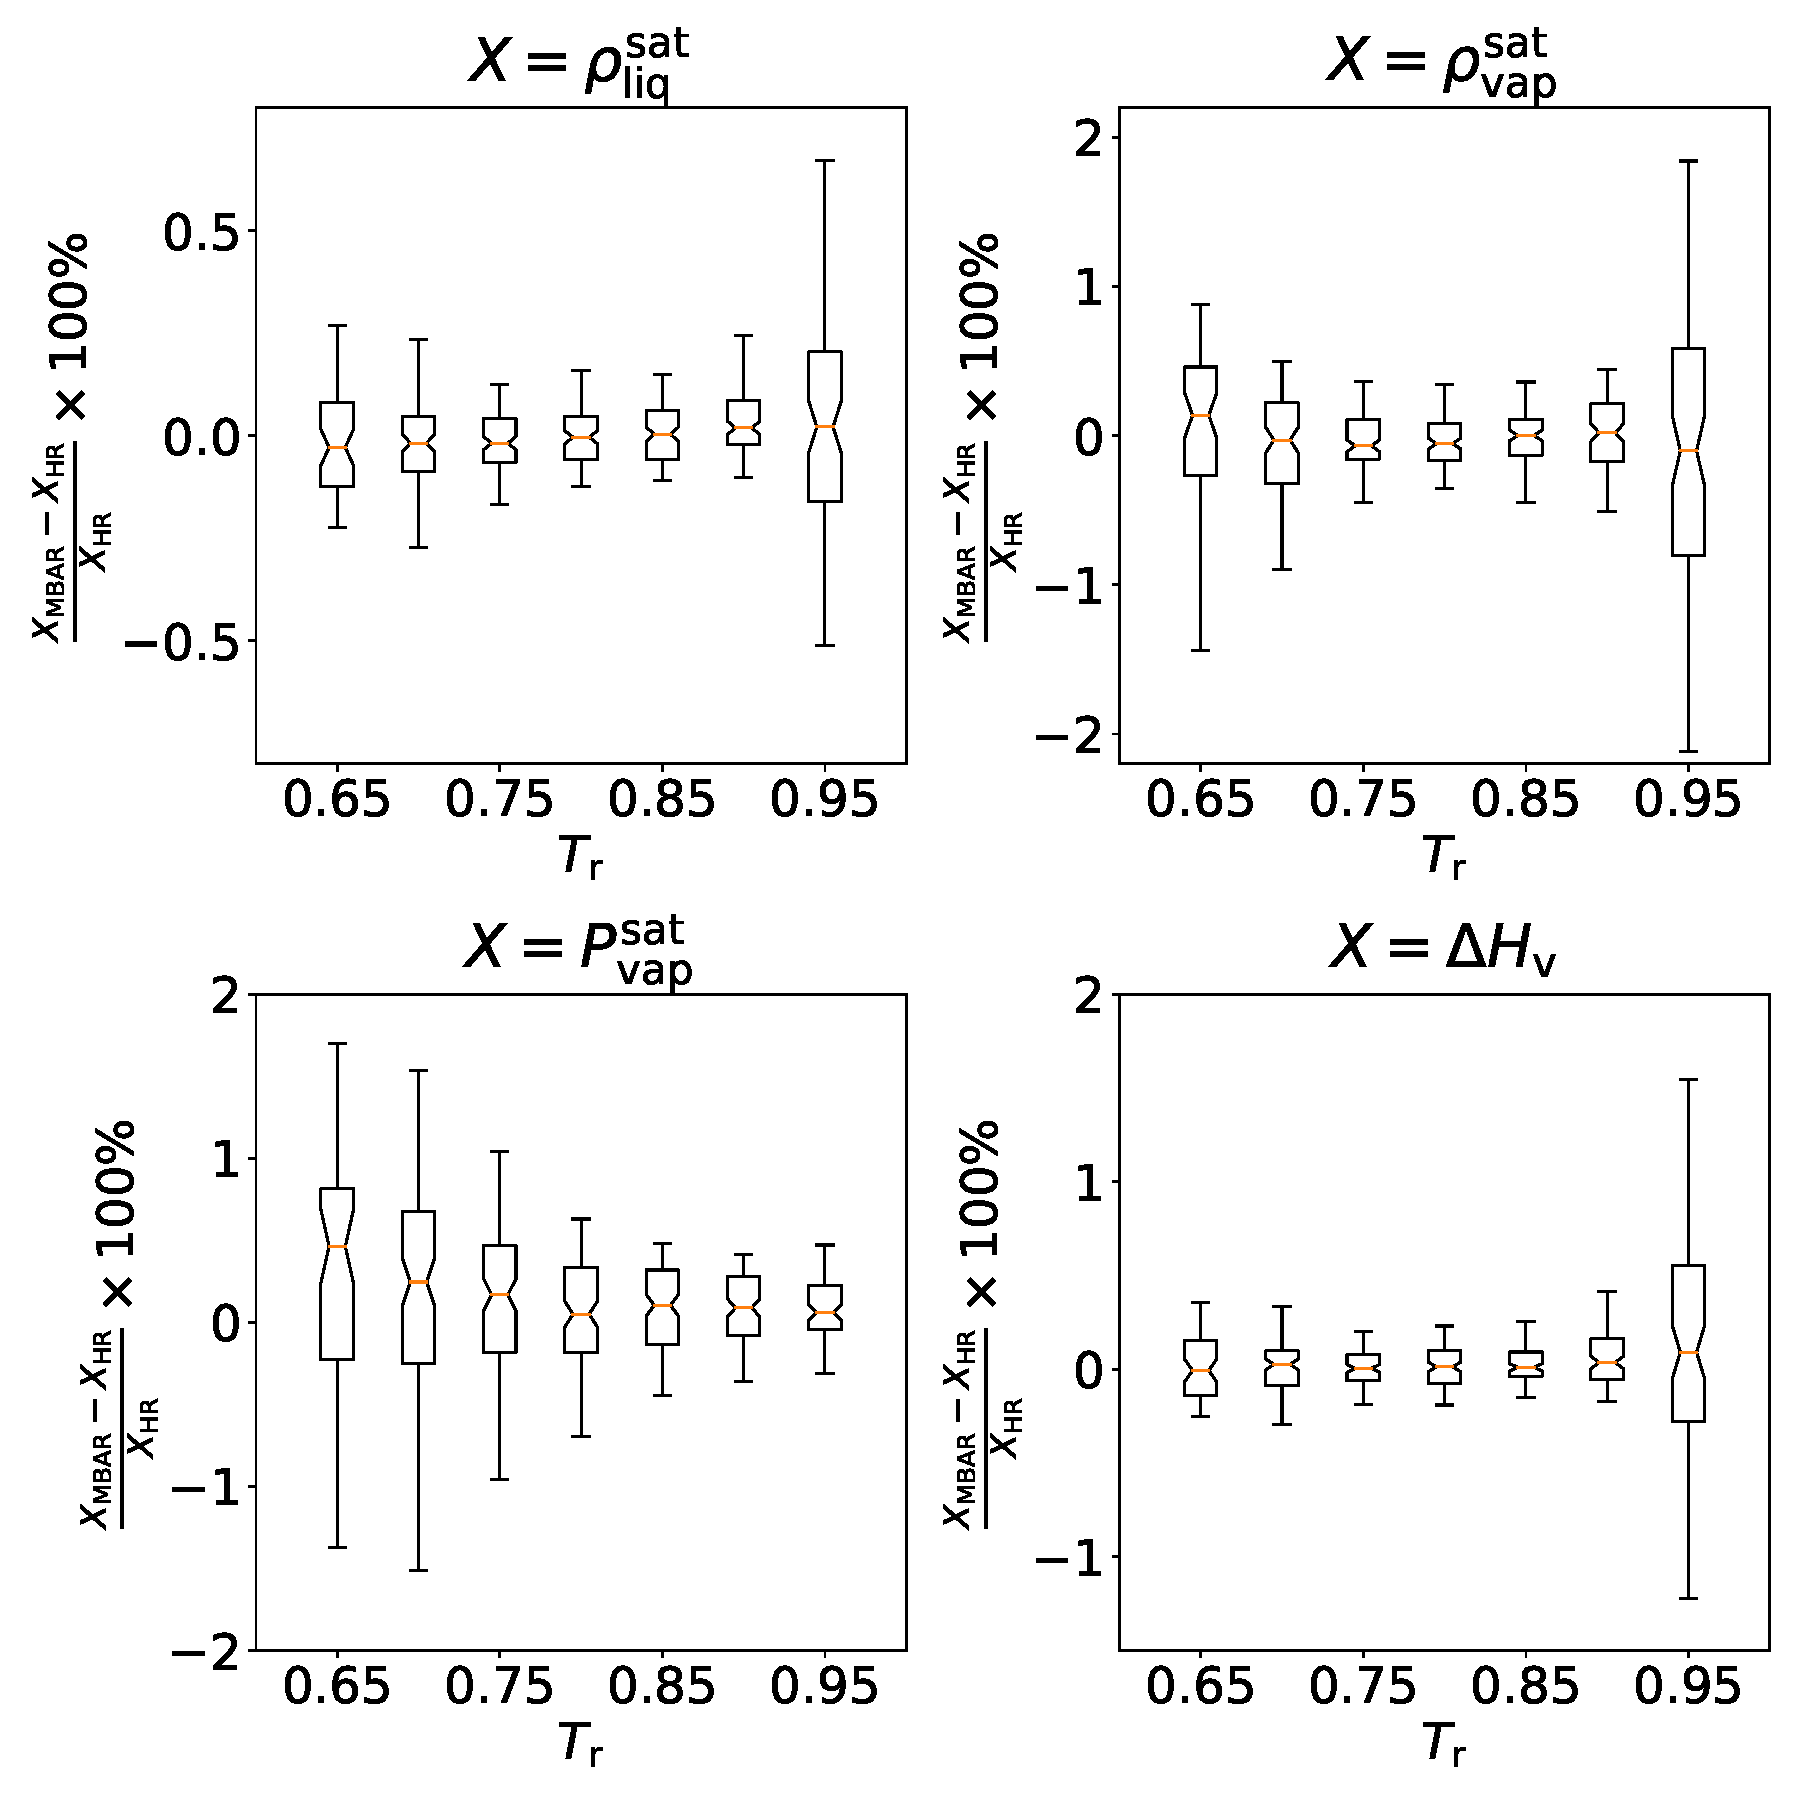
\includegraphics[width=6.4in]{Comparison_MBAR_HR_boxplot_CI.pdf}
		\caption{Percent deviations between coexistence properties computed using histogram reweighting (HR) and Multistate Bennett Acceptance Ratio (MBAR). The HR and MBAR results are in good agreement, i.e., within a few percent and an average percent deviation of approximately 0\%. Top-left, top-right, bottom-left, and bottom-right panels correspond to saturated liquid density, saturated vapor density, saturated vapor pressure, and enthalpy of vaporization, respectively. Middle line denotes the median deviation, boxes depict the first and third quartiles, and whiskers represent the range that contains 95\% of the data.}
		\label{fig:comparison MBAR HR}
	\end{figure}

%(a), (b), (c), and (d)

\subsection{$\epsilon_{\rm rr} = \psi \times \epsilon_{\rm ref}$} \label{sec: eps scaling}

%Figure \ref{fig:epsilon_scaling} presents the $\epsilon$-scaling results for 8 branched alkanes and 11 alkynes using the MiPPE force field as the initial force field. For consistency with the original MiPPE optimization, we use the same scoring function for the branched alkanes and alkynes as Mick et al. and Barhaghi et al., respectively
%\begin{multline} \label{eq: Score}
%S= \frac{1}{N_{\rm exp}} [ w_0 \sum_{j=0}^{N_{\rm exp}} APD(\rho_{\rm liq}^{\rm sat}(T^{\rm sat}_j)) + w_1 \sum_{j=0}^{N_{\rm exp}} APD(\rho_{\rm vap}^{\rm sat}(T^{\rm sat}_j)) \\ + w_2 \sum_{j=0}^{N_{\rm exp}} APD(P_{\rm vap}^{\rm sat}(T^{\rm sat}_j)) + w_3 \sum_{j=0}^{N_{\rm exp}} APD(\Delta H_{\rm v} (T^{\rm sat}_j)) \\ + w_4 \sum_{j=0}^{N_{\rm exp}} \frac{d APD(\rho_{\rm liq}^{\rm sat}(T^{\rm sat}_j))}{dT} + w_5 \sum_{j=0}^{N_{\rm exp}} \frac{d APD(\rho_{\rm vap}^{\rm sat}(T^{\rm sat}_j))}{dT} \\ + w_6 \sum_{j=0}^{N_{\rm exp}} \frac{d APD(P_{\rm vap}^{\rm sat}(T^{\rm sat}_j))}{dT} + w_7 \sum_{j=0}^{N_{\rm exp}} \frac{d APD(\Delta H_{\rm v} (T^{\rm sat}_j))}{dT} ]
%\end{multline}
%where $S$ is the scoring function, $N_{\rm exp}$ is the number of experimental data points, $w_{x}$ are the weights for property $x$, $T^{\rm sat}_j$ are the saturation temperatures for data point $j$, and the absolute percent deviation $(APD)$ is defined as
%\begin{equation} \label{eq: APD}
%APD(X) = \left| \frac{X_{\rm sim} - X_{\rm exp}}{X_{\rm exp}} \right| \times 100 \% 
%\end{equation}
%where $X_{\rm sim}$ and $X_{\rm exp}$ correspond to the respective simulation and (pseudo-) experimental values for property $X$ (e.g., $\rho_{\rm liq}^{\rm sat}$). Note that the weights $(w_x)$ are different for branched alkanes and alkynes, specifically, $w_x = $ (0.6135, 0.0123, 0.2455, 0.0245, 0.0613, 0.0061, 0.0245, 0.0123) and $w_x = $ (0.757, 0, 0.152, 0, 0.076, 0, 0.015, 0) for branched alkanes and alkynes, respectively.
%
%In accordance with the work of Mick et al. and Barhaghi et al., the target values $(X_{\rm exp})$ are computed with pseudo-experimental correlations. The alkyne correlations are from the Design Institute for Physical Properties (DIPPR) while the branched alkane correlations are from the National Institute of Standards and Technology (NIST) Reference Fluid Properties (REFPROP) database.

% Reference Properties (REFPROP) values) are  alkyne target values are the same as those used by Barhaghi et al., namely, they are computed with pseudo-experimental correlations from the Design Institute for Physical Properties (DIPPR). The branched alkane target values are computed with  also the same as Mick et al.

Figure \ref{fig:epsilon_scaling} presents the $\epsilon$-scaling results for 8 branched alkanes and 11 alkynes using the MiPPE-SL force field as $\theta_{\rm ref}$ $(\psi = 1)$. Figure \ref{fig:epsilon_scaling} shows that the alkynes require a greater degree of scaling than the branched alkanes. Weigler et al. tend to characterize the individualization as being useful when the scaling is greater than 0.4\% (i.e., $|1 - \psi| > 0.004$). With this rationale, 3-methylpentane is the only branched alkane that merits $\epsilon$-scaling with the MiPPE-SL force field. Similarly, the TAMie force field also found $\psi \approx 1$ for all branched alkanes, except 3-methylpentane. Although $\psi$ values for iTAMie were not reported for alkynes, the largest $\psi$ value for olefins, ethers, and ketones was $\approx 1.01$. A truly transferable force field should have $\psi \approx 1$ for all compounds. Therefore, the transferability of the MiPPE force field appears to be slightly poorer for 2-pentyne and 2-hexyne, which have an optimized $\psi > 1.01$. 

It is also interesting that only 3 out of 19 compounds require $\psi < 1$. Thus, the well-depths appear to be slightly underestimated by the MiPPE force field. By contrast, this trend was not observed in Reference \citenum{Weidler2018} for TAMie. Also, note that branched alkanes have a pronounced minimum in $S$ with respect to $\psi$, whereas the minimum is more gradual for the alkynes. We attribute this to the fact that the alkynes do not include $\Delta H_{\rm v}$ (a property that depends strongly on $\epsilon$) in the scoring function, i.e., $w_4 = 0$ and $w_7 = 0$. 

%.  is introduced should result in low deviations between experiment and simulation, it is likely that such a parameter set would be overfit and, thus, perform poorly some compounds have sufficient experimental 

	\begin{figure}[htb!]
		\centering
		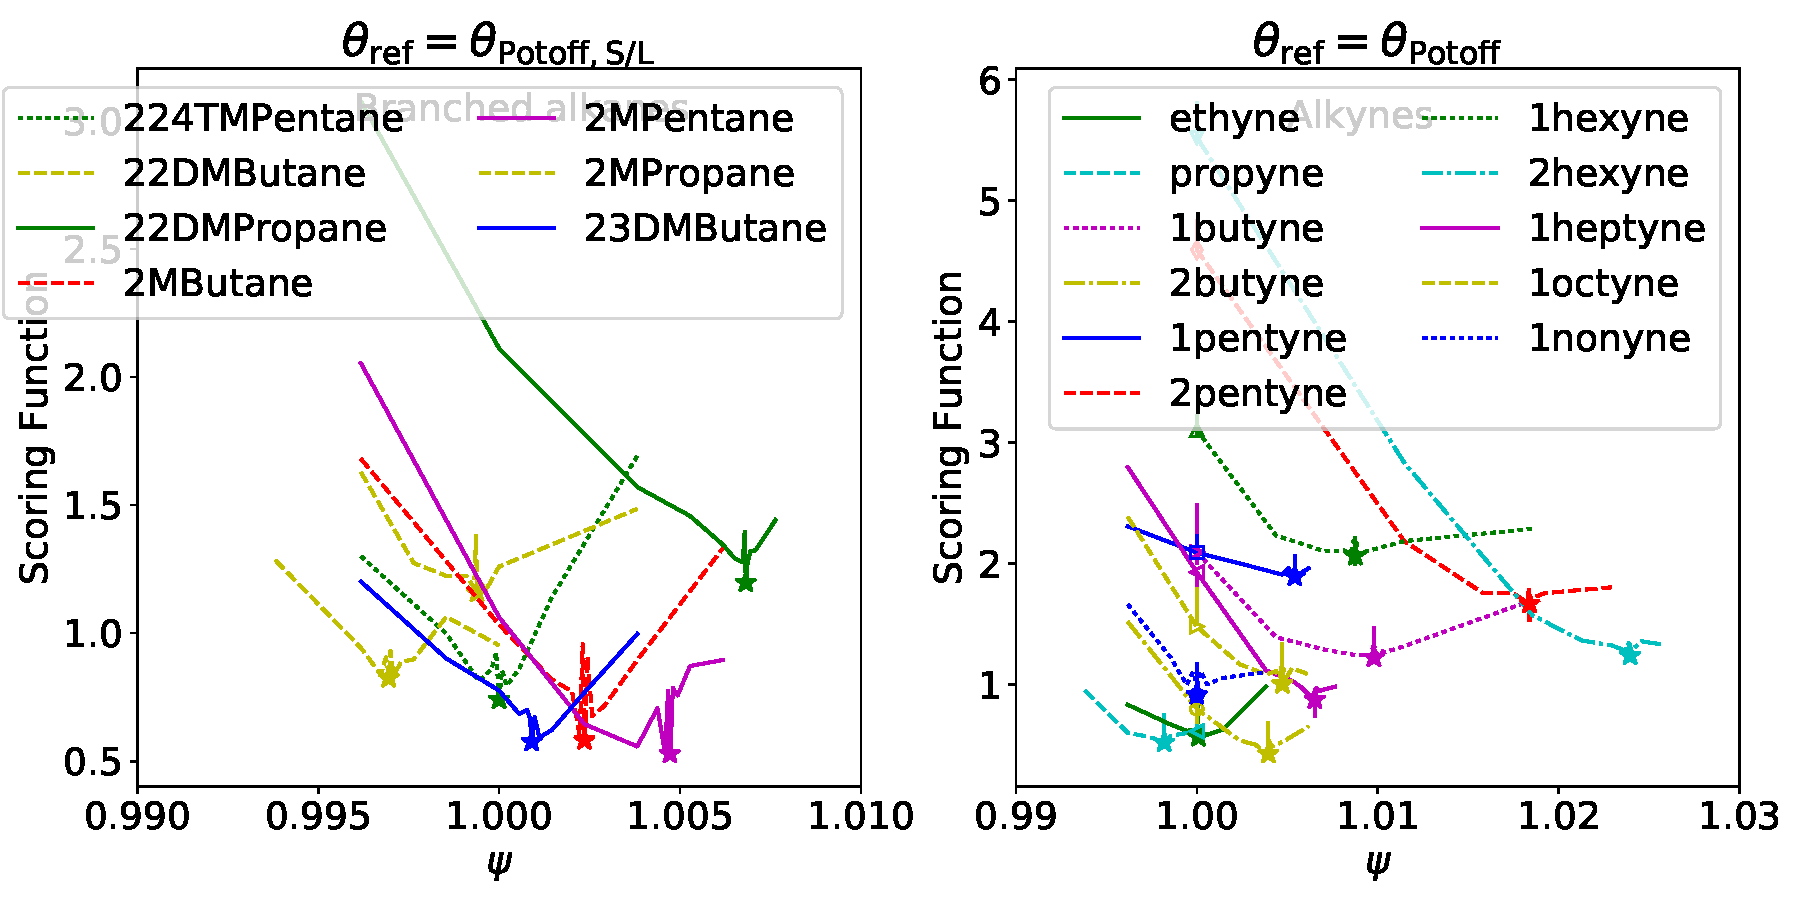
\includegraphics[width=6.4in]{Optimal_epsilon_scaling.pdf}
		\caption{One dimensional optimization with $\epsilon$-scaling $(\psi)$ of MiPPE-SL for select branched alkanes (left) and alkynes (right). MBAR enables prediction of scoring function over range of $\psi$ from configurations that were sampled with $\psi = 1$ (dashed line). Open symbols correspond to the optimal $\psi$ value for a given compound.}
		\label{fig:epsilon_scaling}
	\end{figure}

% MBAR is ideally suited for $\epsilon$-scaling for at least two reasons.
 
%At least two reasons exist for why MBAR is ideally suited for $\epsilon$-scaling. First, the energies in Equation \ref{BLANK} can be scaled by $\psi$ such that the configurations do not need to be stored or recomputed. Second, MBAR is more reliable for changes in $\epsilon$ rather than changes in $\sigma$ and/or $\lambda$ \cite{Postdoc_1}. 

\subsection{$\epsilon_{\rm ref} \neq \epsilon_{\rm rr}$, $\sigma_{\rm ref} \neq \sigma_{\rm rr}$, and $\lambda_{\rm ref} \neq \lambda_{\rm rr}$} \label{sec: litFF}

A more demanding test of GCMC-MBAR than $\epsilon$-scaling is to vary several non-bonded parameters simultaneously, including $\sigma$ and $\lambda$. Because it is not possible to visualize a parameter space of greater than three dimensions, we perform this analysis of GCMC-MBAR using the TraPPE, NERD, MiPPE-gen, and MiPPE-SL force fields. Specifically, we utilize GCMC-MBAR to predict coexistence properties for the NERD and MiPPE-SL force fields using configurations sampled from TraPPE and MiPPE-gen, respectively (see Figure \ref{fig:refFF_to_rrFF_lam_constant}). We also use GCMC-MBAR to predict coexistence properties for the TraPPE force field by sampling configurations with MiPPE-gen, and vice versa (see Figure \ref{fig:refFF_to_rrFF_lam12to16}). 

Note that all three non-bonded parameters ($\epsilon$, $\sigma$, and $\lambda$) for all four united-atom types (CH$_3$, CH$_2$, CH, and C) are different between the TraPPE and MiPPE-gen force fields. The TraPPE and NERD $\epsilon$ and $\sigma$ values are different for all four united-atom types while $\lambda = 12$ for both force fields. The MiPPE-gen and MiPPE-SL force fields only differ in the $\epsilon$ and/or $\sigma$ values for the CH and C sites. However, the difference in $\epsilon$ and $\sigma$ values for MiPPE-gen and MiPPE-SL is significantly smaller than that between TraPPE and NERD. Therefore, the MiPPE-gen $\Rightarrow$ MiPPE-SL results correspond to $\theta_{\rm rr} \approx \theta_{\rm ref}$, which is important when fine-tuning a pre-optimized force field.

%Specifically, the 2-methylpropane and 2,3-dimethylbutane parameters are the same except for $\sigma_{\rm CH}$, the 2,2-dimethylpropane parameters are the same except for $\epsilon_{\rm C}$, the 2,3,4-trimethylpentane parameters are the same except for $\epsilon_{\rm CH}$ and $\sigma_{\rm CH}$, and the 2,2,4-trimethylpentane parameters are the same except for $\epsilon_{\rm CH}$, $\sigma_{\rm CH}$, and $\sigma_{\rm C}$.

Figures \ref{fig:refFF_to_rrFF_lam_constant} and \ref{fig:refFF_to_rrFF_lam12to16} compare the GCMC-MBAR predicted values for $\theta_{\rm rr} \neq \theta_{\rm ref}$ to the literature GCMC-HR values obtained by direct simulation. Figure \ref{fig:refFF_to_rrFF_lam_constant} contains $\lambda_{\rm rr} = \lambda_{\rm ref}$ while Figure \ref{fig:refFF_to_rrFF_lam12to16} corresponds to $\lambda_{\rm rr} \neq \lambda_{\rm ref}$. As observed in Figures \ref{fig:refFF_to_rrFF_lam_constant} and \ref{fig:refFF_to_rrFF_lam12to16}, MBAR is extremely reliable at predicting vapor phase properties ($\rho_{\rm vap}^{\rm sat}$ and $P_{\rm vap}^{\rm sat}$). GCMC-MBAR is remarkably accurate at predicting liquid phase properties ($\rho_{\rm liq}^{\rm sat}$ and $\Delta H_{\rm v}$, which depends on both phases) even for the fairly significant differences in the TraPPE and NERD $\sigma$ values. However, Figure \ref{fig:refFF_to_rrFF_lam12to16} shows that GCMC-MBAR is less reliable for liquid phase properties when $\lambda_{\rm rr} \neq \lambda_{\rm ref}$. This undesirable behavior can be explained by the low number of effective snapshots in the liquid phase.

%In particular, note that the $\rho_{\rm liq}^{\rm sat}$ estimates in Figure \ref{fig:refFF_to_rrFF_lam12to16} are sporadic and unreliable.

%, which demonstrates that the repulsive exponent $(\lambda)$ greatly impacts the configurational overlap in the liquid phase but not the vapor phase. The poor overlap when varying $\lambda$ is consistent with the MBAR-ITIC results \cite{Postdoc_1}. However, GCMC-MBAR provides considerable improvement in predicting $P_{\rm vap}^{\rm sat}$ compared to MBAR-ITIC. For this reaon, we recommend reducing the $\rho_{\rm liq}^{\rm sat}$ weight in the scoring function when varying $\lambda$. The degree to which the weight is reduced should depend on the number of effective samples.


%Because it is not possible to visualize a parameter space of greater than two dimensions, Figures \ref{fig:refFF_to_rrFF_lam_constant} and \ref{fig:refFF_to_rrFF_lam12to16} demonstrate the reliability of MBAR when multiple parameters are varied simultaneously. 

%For example, all three non-bonded parameters ($\epsilon$, $\sigma$, and $\lambda$) for all four united-atom types (CH$_3$, CH$_2$, CH, and C) are different between the TraPPE and Potoff-gen force fields (see Figure \ref{fig:refFF_to_rrFF_lam12to16}). The TraPPE and NERD $\epsilon$ and $\sigma$ values are different for all four united-atom types while $\lambda = 12$ for both force fields (see Figure \ref{fig:refFF_to_rrFF_lam_constant}). The Potoff-gen and Potoff-SL force fields only differ in the $\epsilon$ and/or $\sigma$ values for the CH and C sites (see Figure \ref{fig:refFF_to_rrFF_lam_constant}). Specifically, the 2-methylpropane parameters are identical except for $\sigma_{\rm CH}$, the 2,2-dimethylpropane parameters are the same except for $\epsilon_{\rm C}$, and three parameters are different for 2,2,4-trimethylpentane ($\epsilon_{\rm CH}$, $\sigma_{\rm CH}$, and $\sigma_{\rm C}$). However, the difference in $\epsilon$ and $\sigma$ values for Potoff-gen and Potoff-SL is significantly smaller than that between TraPPE and NERD.

	\begin{figure}[htb!]
		\centering
		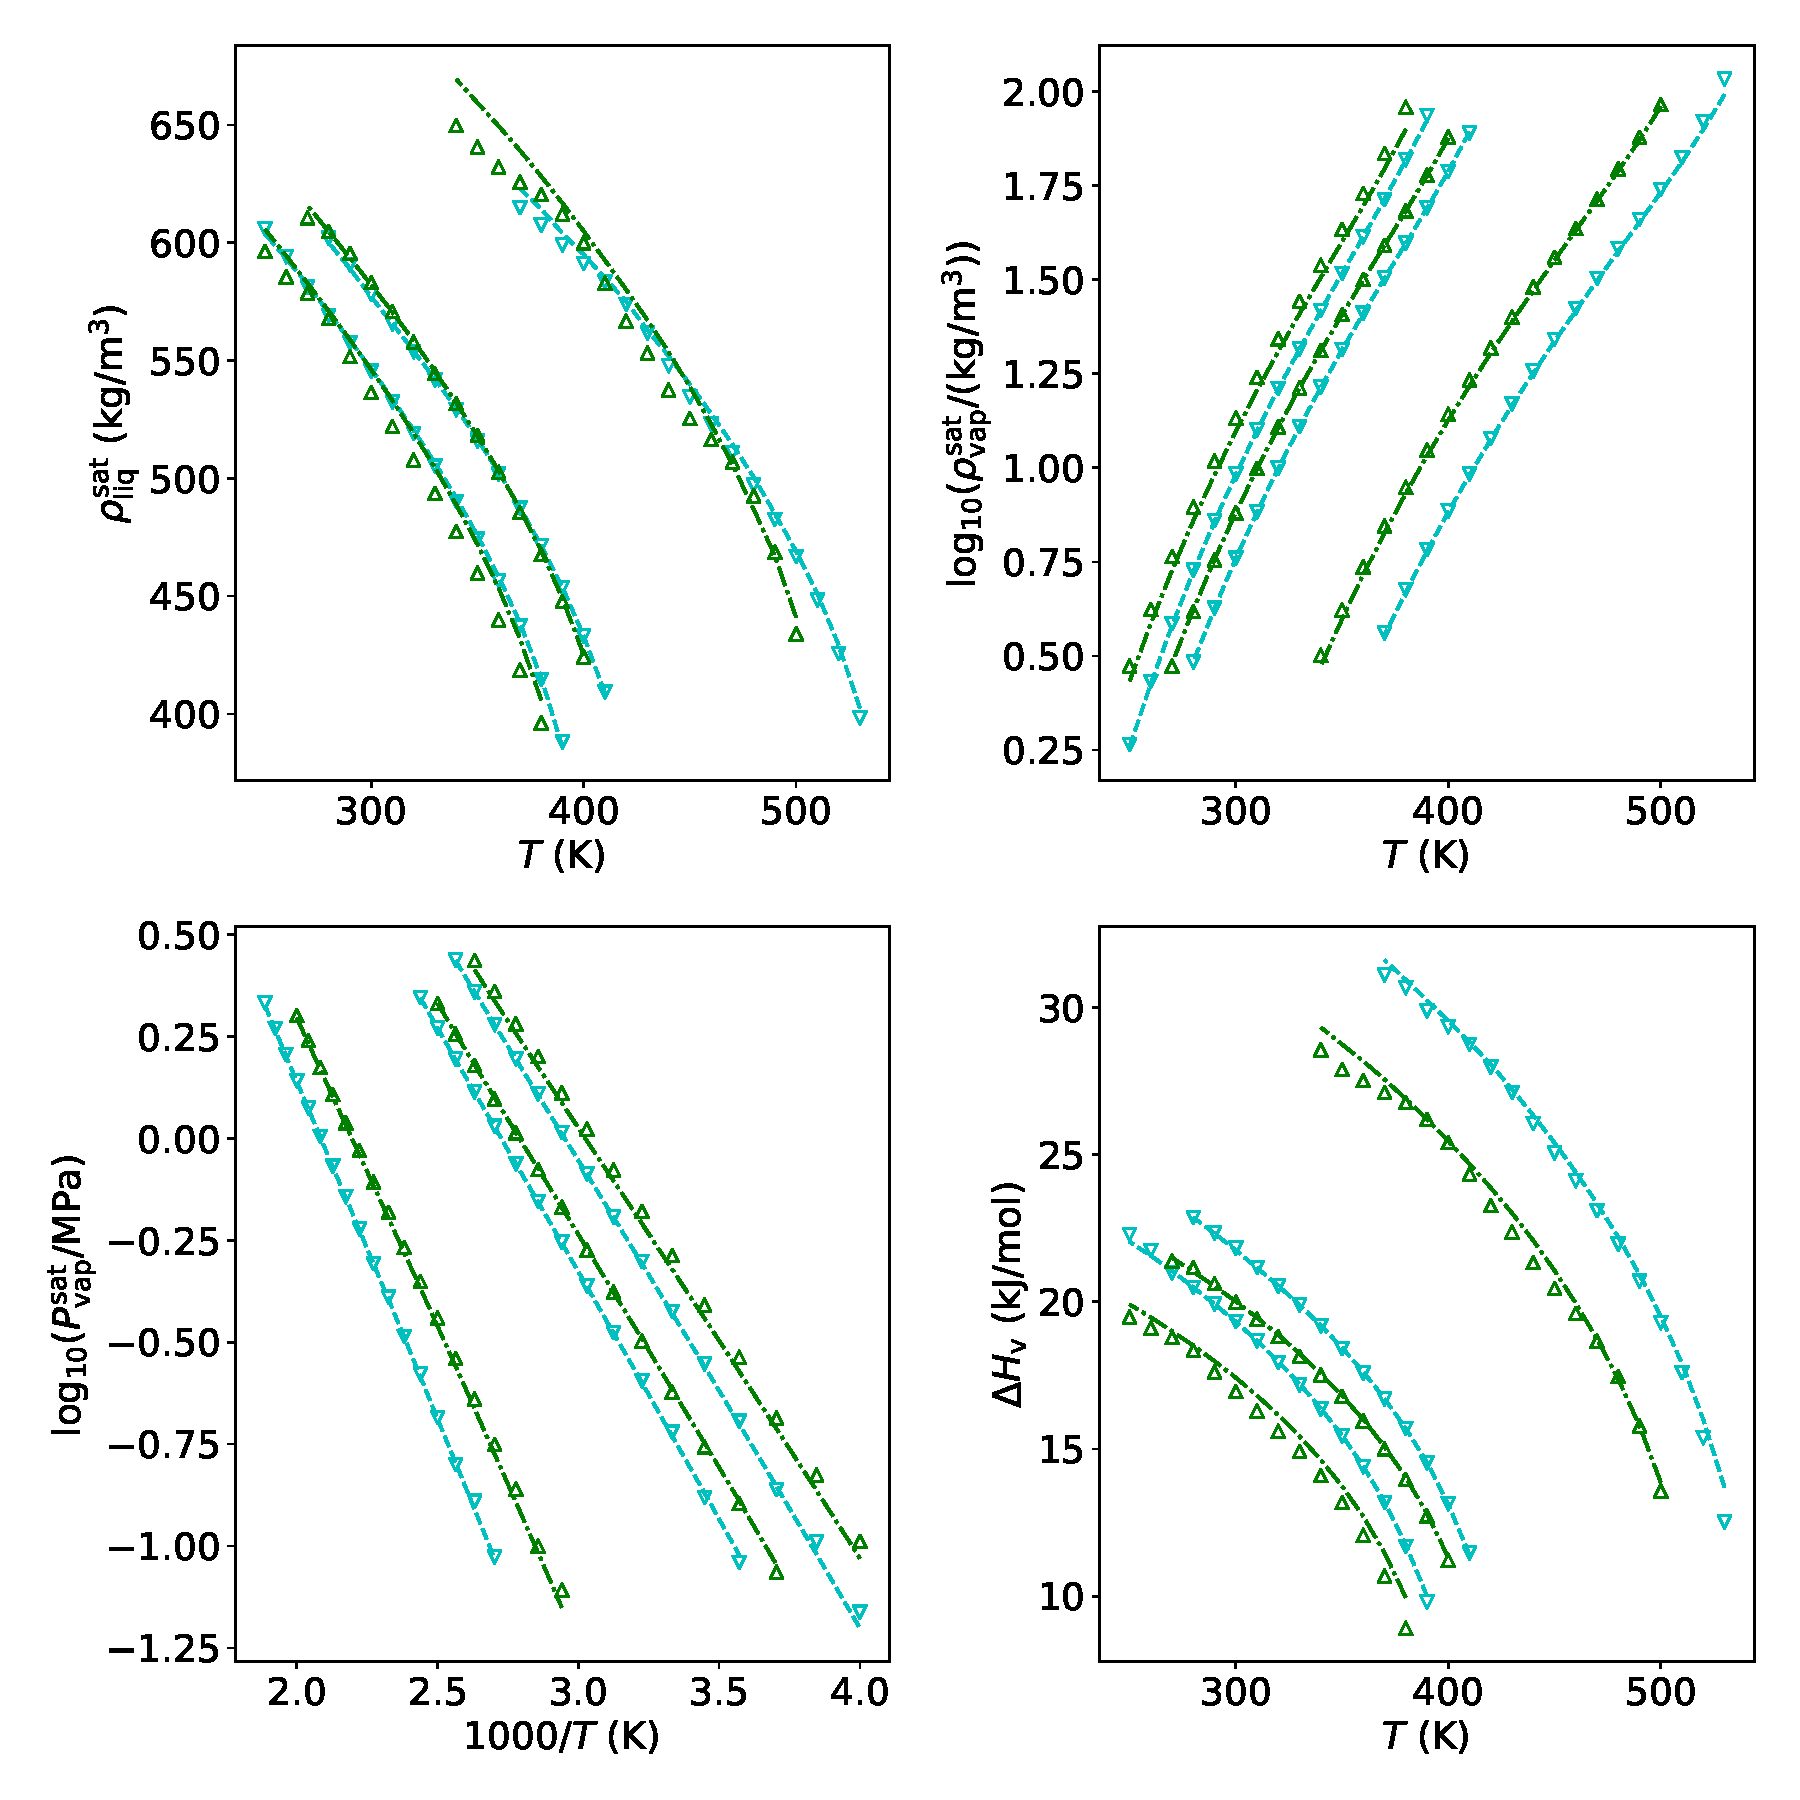
\includegraphics[width=6.4in]{refFF_to_rrFF_lam_constant.pdf}
		\caption{Comparison between MBAR-GCMC estimates (symbols, $\theta_{\rm rr} \neq \theta_{\rm ref}$) and MBAR-HR literature values (lines) with a constant repulsive exponent, i.e., $\lambda_{\rm rr} = \lambda_{\rm ref}$. MBAR predicts both liquid and vapor properties accurately for $\lambda_{\rm rr} = \lambda_{\rm ref}$. MBAR-GCMC estimates for the NERD and MiPPE-SL force fields are computed using configurations sampled from TraPPE and MiPPE-gen, respectively. Top-left, top-right, bottom-left, and bottom-right panels correspond to saturated liquid density, saturated vapor density, saturated vapor pressure, and enthalpy of vaporization, respectively.}
		\label{fig:refFF_to_rrFF_lam_constant}
	\end{figure}

	\begin{figure}[htb!]
		\centering
		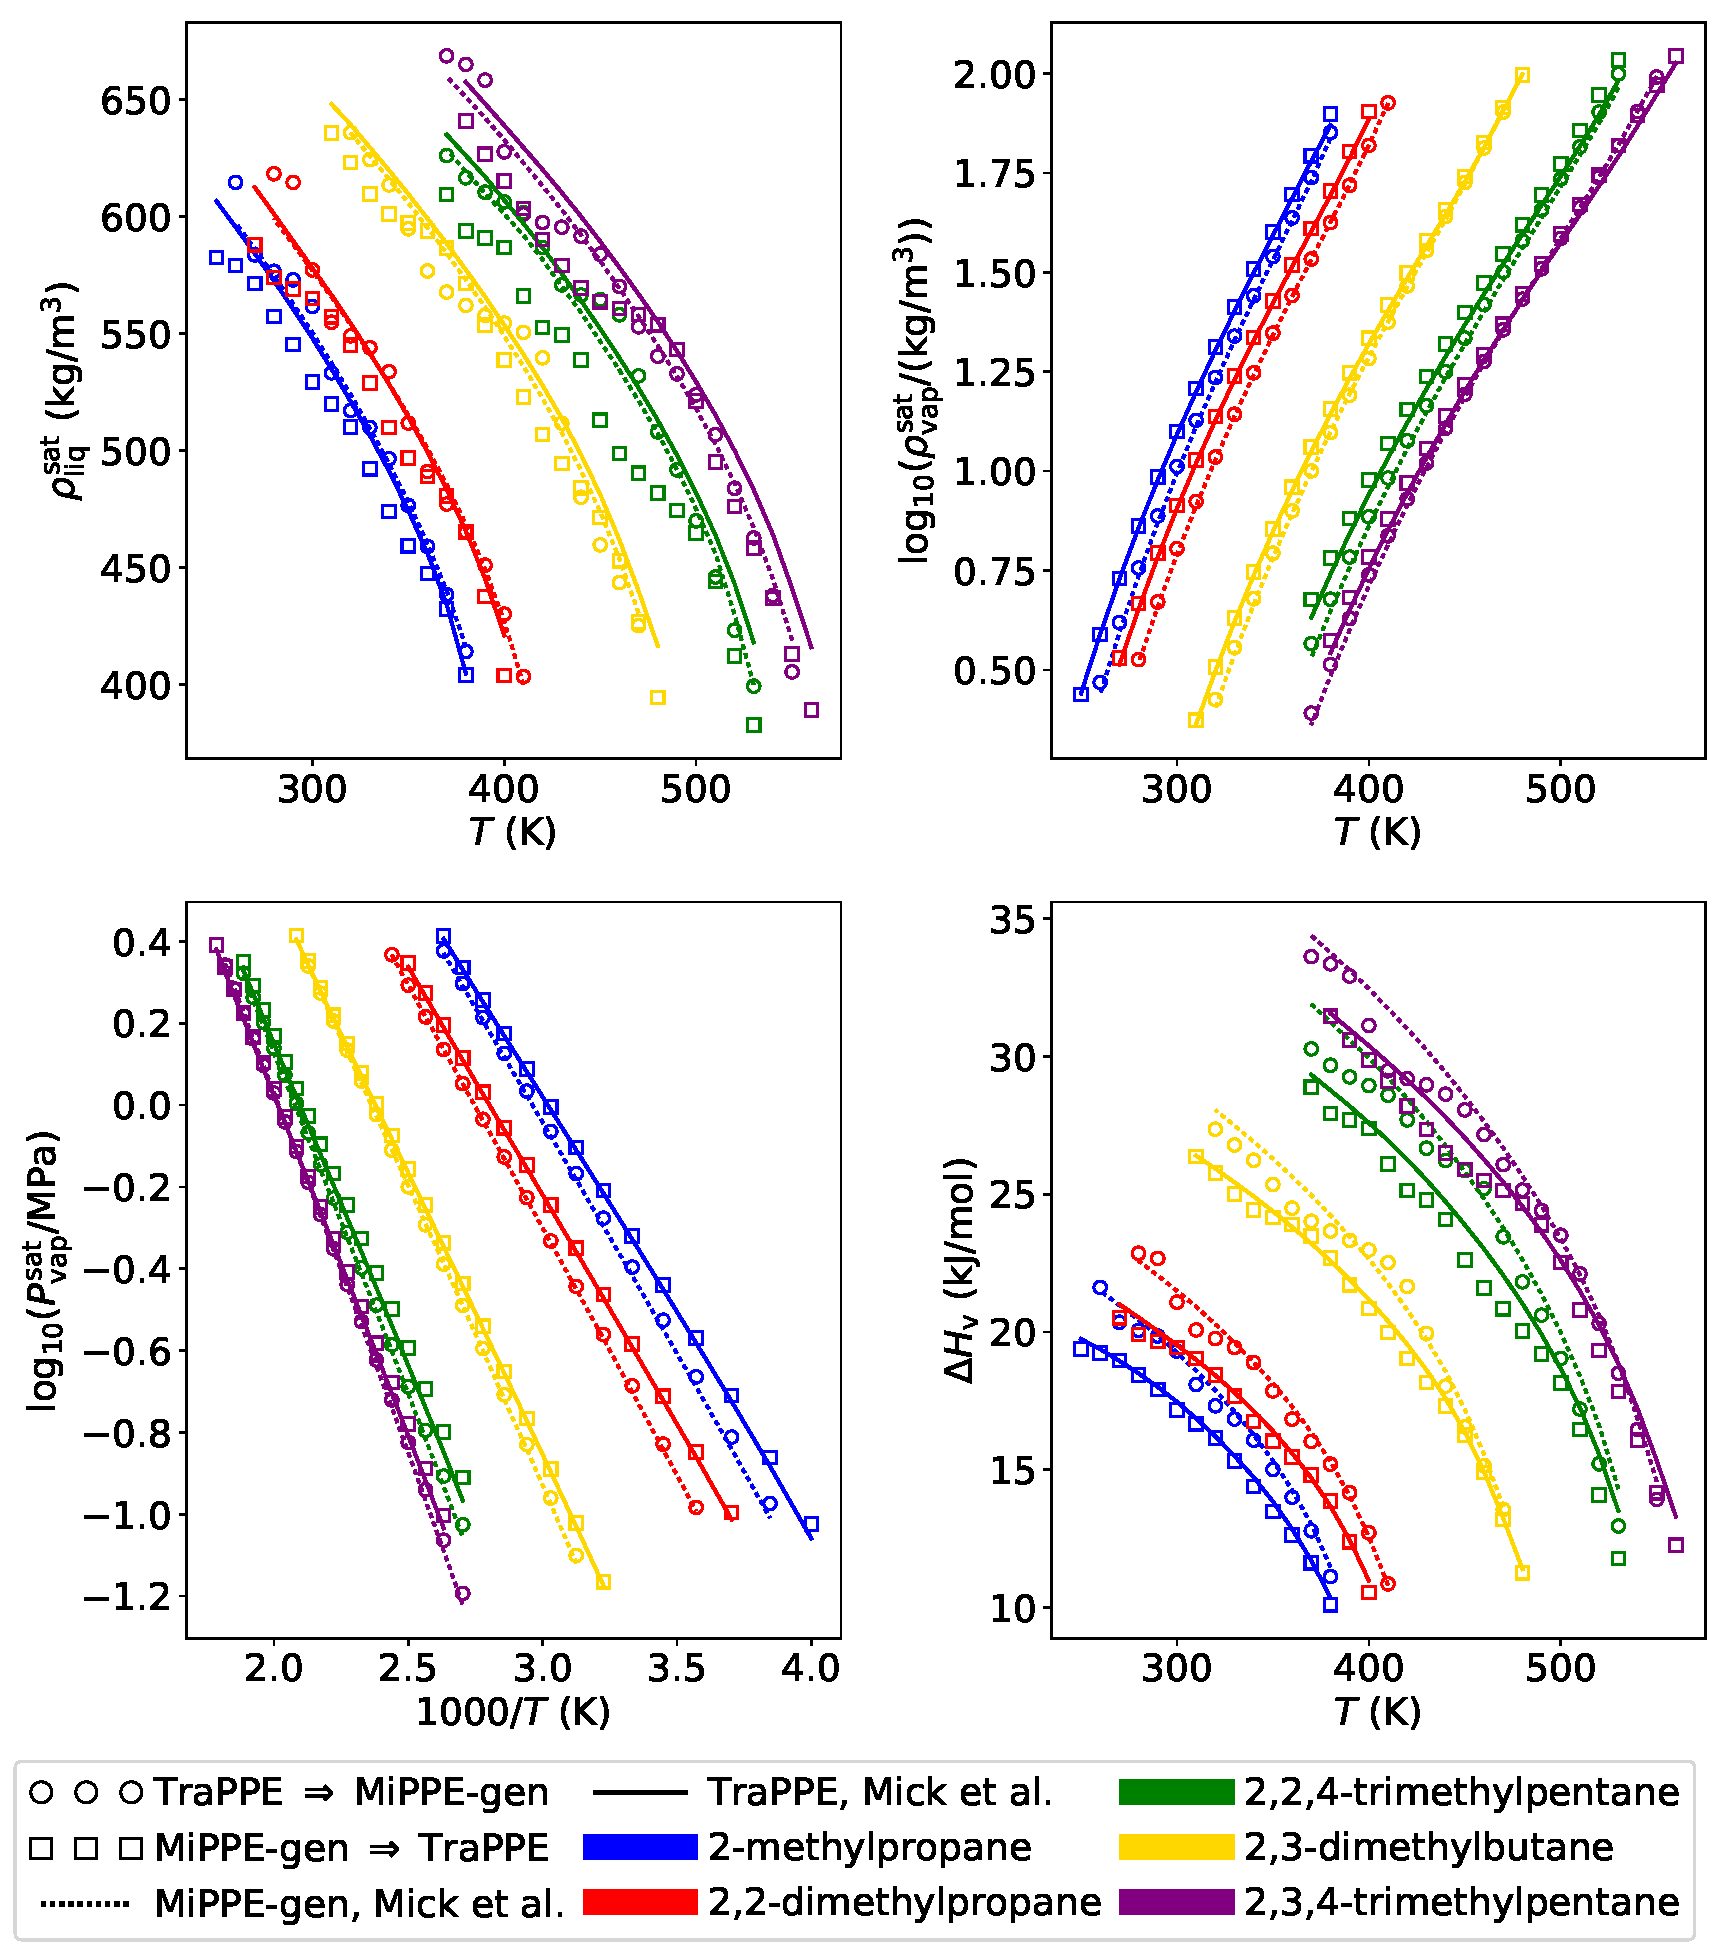
\includegraphics[width=6.4in]{refFF_to_rrFF_lam_12to16.pdf}
		\caption{Comparison between MBAR-GCMC estimates (symbols, $\theta_{\rm rr} \neq \theta_{\rm ref}$) and MBAR-HR literature values (lines) with a non-constant repulsive exponent, i.e., $\lambda_{\rm rr} \neq \lambda_{\rm ref}$. MBAR predicts only vapor properties accurately for $\lambda_{\rm rr} \neq \lambda_{\rm ref}$. MBAR-GCMC estimates for the TraPPE force field are computed using configurations sampled from MiPPE-gen, and vice versa. Top-left, top-right, bottom-left, and bottom-right panels correspond to saturated liquid density, saturated vapor density, saturated vapor pressure, and enthalpy of vaporization, respectively.}
		\label{fig:refFF_to_rrFF_lam12to16}
	\end{figure}

Figure \ref{fig:Neff} demonstrates that $K_{\rm snaps}^{\rm eff}$ is typically much greater in the vapor phase than in the liquid phase. Messerly et al. report that MBAR-ITIC is reliable if $K_{\rm snaps}^{\rm eff} > 50$. Applying this heuristic to GCMC-MBAR helps qualify why the liquid properties are poorly estimated in some systems while the vapor properties are much more accurate. Specifically, $K_{\rm snaps}^{\rm eff}$ is less than $50$ in the liquid phase when $\lambda_{\rm rr} \neq \lambda_{\rm ref}$ (TraPPE $\Leftrightarrow$ MiPPE-gen) while it is typically greater than 50 for $\lambda_{\rm rr} = \lambda_{\rm ref}$ (MiPPE-gen $\Rightarrow$ MiPPE-SL and TraPPE $\Rightarrow$ NERD).

% while  is much greater in the liquid phase than the vapor phase.  if the overlap between systems is sufficient for MBAR to be reliable.  is 

The poor overlap when varying $\lambda$ is consistent with the MBAR-ITIC results \cite{Postdoc_1}. However, GCMC-MBAR provides considerable improvement in predicting $\rho_{\rm vap}^{\rm sat}$ and $P_{\rm vap}^{\rm sat}$ compared to what was previously observed for MBAR-ITIC. For this reason, we recommend reducing the $\rho_{\rm liq}^{\rm sat}$ and $\Delta H_{\rm v}$ weights $(w_0$, $w_3$, $w_4$, and $w_7)$ in the scoring function (Equation \ref{eq: Score}) when varying $\lambda$. The degree to which the weight is reduced should depend on the number of effective samples $(K_{\rm snaps}^{\rm eff})$.

	\begin{figure}[htb!]
		\centering
		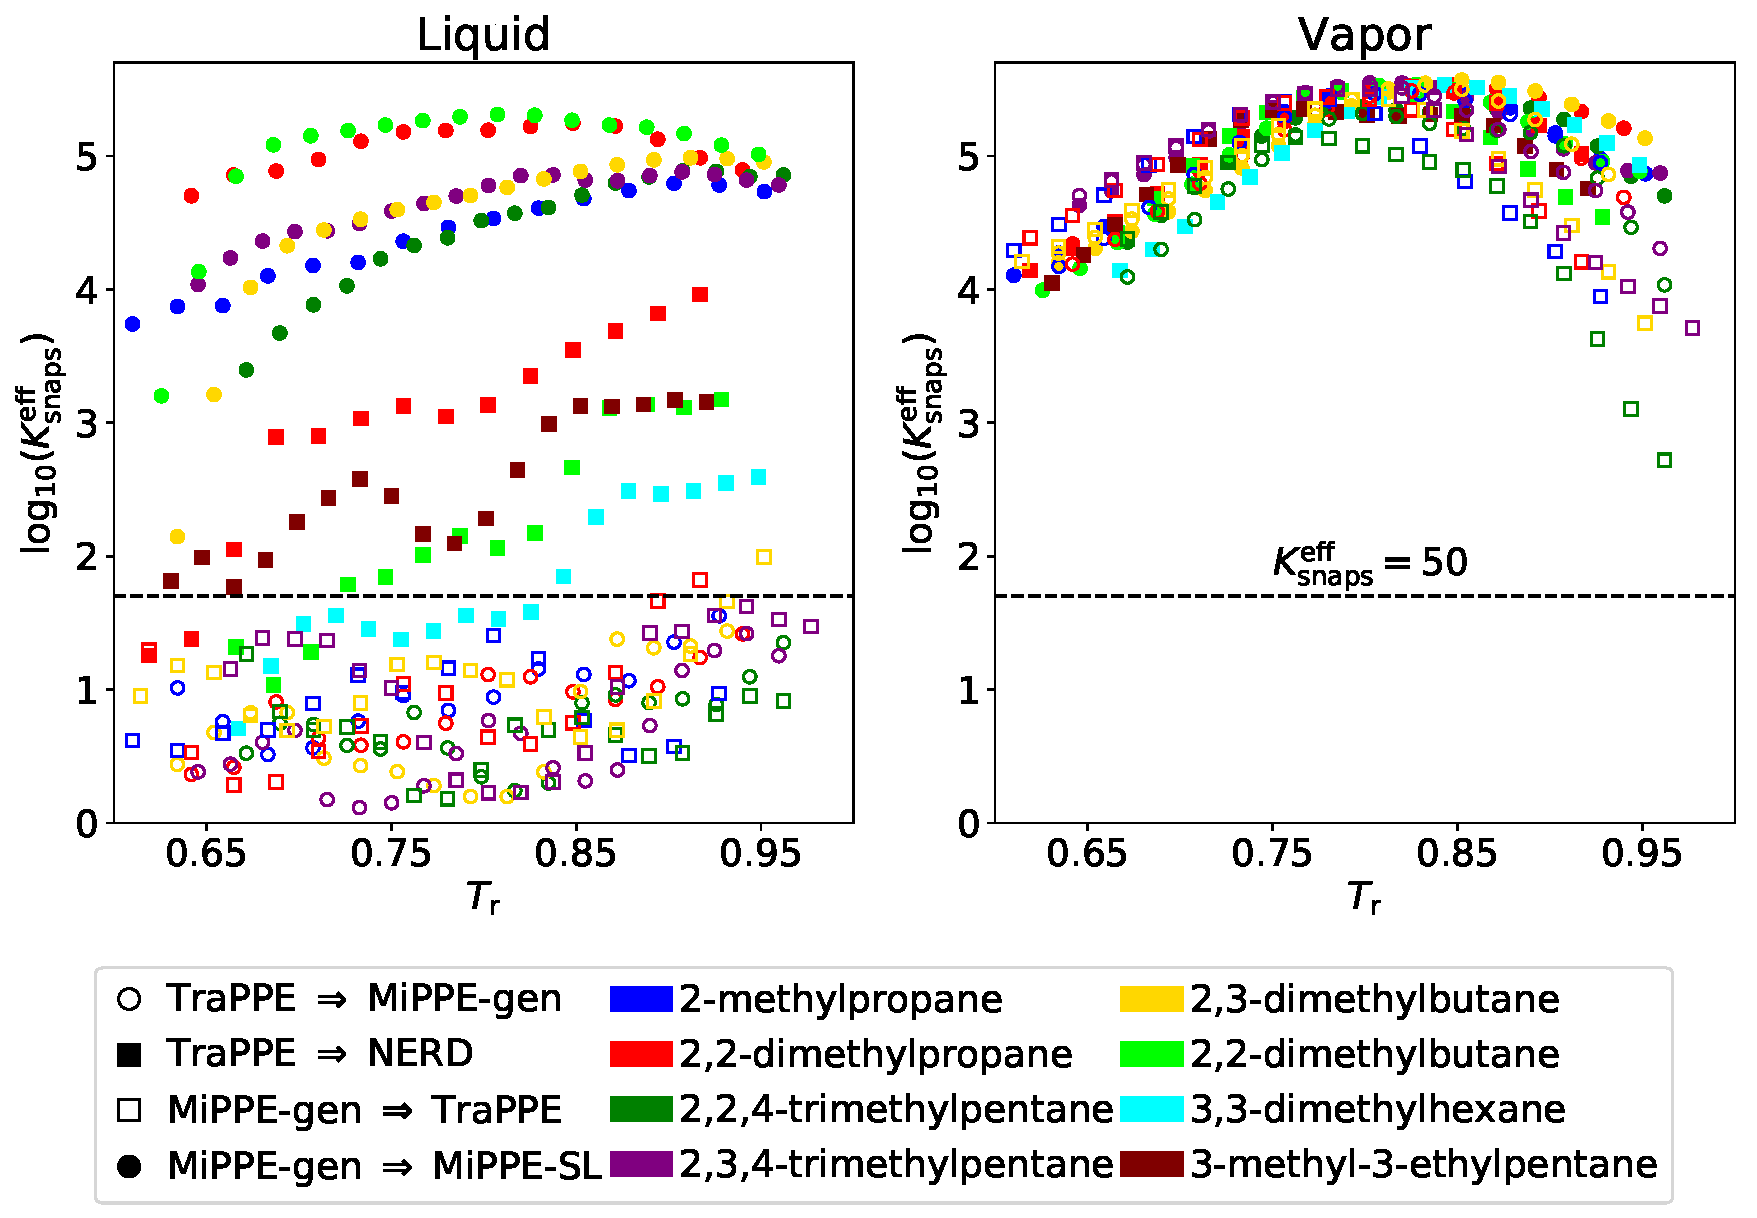
\includegraphics[width=6.4in]{refFF_to_rrFF_Neff_alt.pdf}
		\caption{Number of effective snapshots $(K_{\rm snaps}^{\rm eff})$ in the liquid (left panel) and vapor (right panel) phases. Good overlap $(K_{\rm snaps}^{\rm eff} \gg 50)$ is achieved in the vapor phase for each system while poor overlap in liquid phase $(K_{\rm snaps}^{\rm eff} < 50)$ is observed for $\lambda_{\rm rr} \neq \lambda_{\rm ref}$. Color scheme is the same as Figures \ref{fig:refFF_to_rrFF_lam_constant} and \ref{fig:refFF_to_rrFF_lam12to16}. Closed and open symbols correspond to $\lambda_{\rm rr} = \lambda_{\rm ref}$ and $\lambda_{\rm rr} \neq \lambda_{\rm ref}$, respectively.}
		\label{fig:Neff}
	\end{figure} 

\subsection{Case Study: Optimizing cyclohexane Mie $\lambda$-6 parameters} \label{sec: Case study}

We have demonstrated that GCMC-MBAR is accurate when $K_{\rm snaps}^{\rm eff} \gg 50$, which is typically the case in the vapor phase and in the liquid phase when $\lambda_{\rm rr} = \lambda_{\rm ref}$. In this section, we present how GCMC-MBAR can rapidly optimize the Mie $\lambda$-6 parameters. We have chosen cyclohexane for this case study as this is a compound for which MiPPE does not yet have non-bonded parameters. Also, because cyclohexane consists of a single united-atom site type, it is a convenient molecule for representing the scoring function in 2-dimensions ($\epsilon_{\rm CH_2}$ and $\sigma_{\rm CH_2}$ for a given value of $\lambda_{\rm CH_2}$).

Figure \ref{fig:Score_CYC6} depicts the scoring function for different values of $\epsilon_{\rm CH_2}$, $\sigma_{\rm CH_2}$, and $\lambda_{\rm CH_2}$ as a heat map, where red denotes the optimal parameter set (i.e., the lowest values of $S$.) Similar figures have been reported in the literature using GCMC-HR \cite{Potoff_branched,Barhaghi2017}. The key difference is that the heat maps reported in the literature were obtained by performing GCMC simulations with each value of $\epsilon$, $\sigma$, and $\lambda$. By contrast, the results shown in Figure \ref{fig:Score_CYC6} were obtained by performing GCMC simulations with a single parameter set, namely, the TraPPE parameters (depicted as an ``X'' in Figures \ref{fig:Score_CYC6} and \ref{fig:Neff}). MBAR reweights these same configurations for all other parameter sets. Furthermore, $U(\theta_{\rm rr})$ is computed with basis functions, enabling the GCMC-MBAR recompute step to be extremely fast. 

In this optimization example (a 2-dimensional grid search over integer values of $\lambda$) the GCMC simulations could be run in parallel, which would negate the computational gain of GCMC-MBAR compared with GCMC-HR. However, in general, higher dimensional optimization algorithms are performed in sequence, where each iteration proposes new parameter set(s). In this scenario, GCMC-MBAR (with basis functions) is orders of magnitude faster than the traditional GCMC-HR approach, which would require performing new GCMC simulations for each iteration. 

Note that the TraPPE force field utilizes a Lennard-Jones 12-6 potential (i.e., $\lambda_{\rm TraPPE} = 12$) and, therefore, the results in the top-left panel are for the case where $\lambda_{\rm rr} = \lambda_{\rm ref} = 12$, while the other panels correspond to $\lambda_{\rm rr} \neq \lambda_{\rm ref}$. Figure \ref{fig:Neff_CYC6} shows that, as expected, $K_{\rm snaps}^{\rm eff}$ in the liquid phase are much lower for $\lambda_{\rm rr} \neq \lambda_{\rm ref}$ than for $\lambda_{\rm rr} = \lambda_{\rm ref}$. In addition, the smooth contours in Figure \ref{fig:Score_CYC6} for $\lambda_{\rm rr} = \lambda_{\rm ref} = 12$ and the wide range of parameters over which $\bar K_{\rm snaps}^{\rm eff, liq} \gg 50$ suggests that GCMC-MBAR is highly reliable for optimizing $\epsilon_{\rm CH_2}$ and $\sigma_{\rm CH_2}$ for a fixed value of $\lambda_{\rm CH_2}$. Even more remarkable is that GCMC-MBAR predicts smooth contours for $\lambda_{\rm rr} \neq \lambda_{\rm ref}$ despite lower values of $\bar K_{\rm snaps}^{\rm eff, liq}$. This demonstrates that GCMC-MBAR is capable of converting a pre-tuned Lennard-Jones 12-6 potential (TraPPE) into a Mie $\lambda$-6 potential without simulating hundreds of different parameter sets.     

	\begin{figure}[htb!]
		\centering
		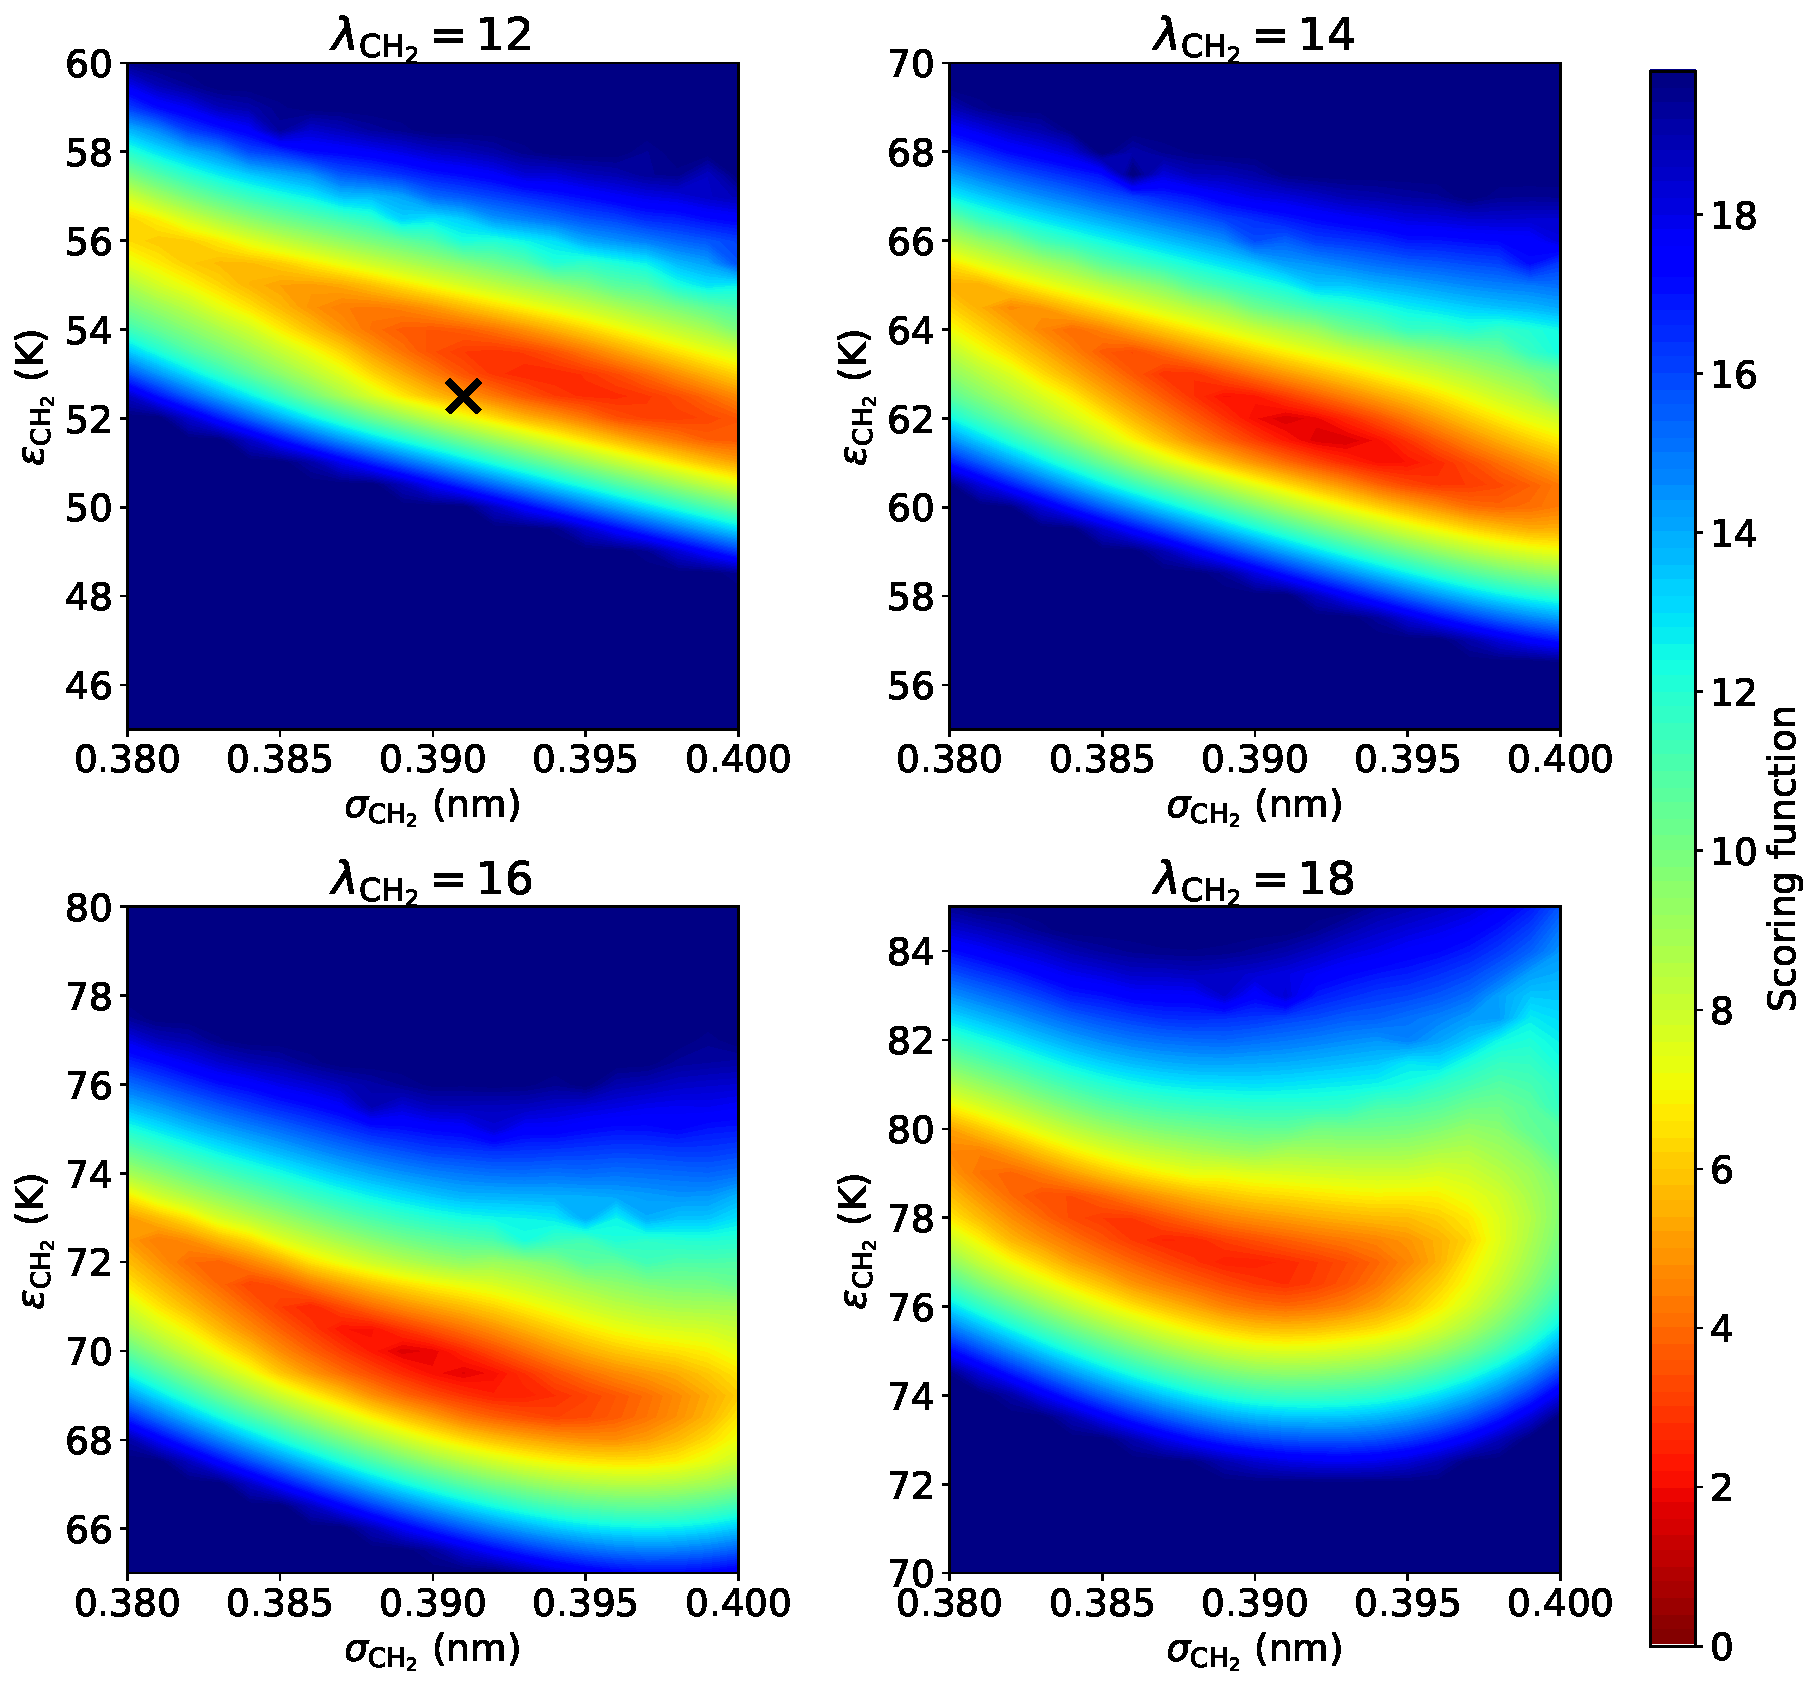
\includegraphics[width=6.4in]{CYC6_scoring_function_lam_alt.pdf}
		\caption{Scoring function values with respect to $\epsilon_{\rm CH_2}$ and $\sigma_{\rm CH_2}$ for cyclohexane. GCMC-MBAR enables rapid optimization of Mie $\lambda$-6 parameters from a single reference force field $(\theta_{\rm ref} = \theta_{\rm TraPPE}$, depicted as a black ``X''). Top-left, top-right, bottom-left, and bottom-right panels correspond $\lambda_{\rm CH_2} = 12$, $\lambda_{\rm CH_2} = 14$, $\lambda_{\rm CH_2} = 16$, $\lambda_{\rm CH_2} = 18$, respectively. Red denotes the optimal parameter set, i.e., the lowest value of $S$.}% White star represents the optimal parameter set, i.e., the lowest value of $S$, for a given $\lambda_{\rm CH_2}$.}
		\label{fig:Score_CYC6}
	\end{figure} 

	\begin{figure}[htb!]
		\centering
		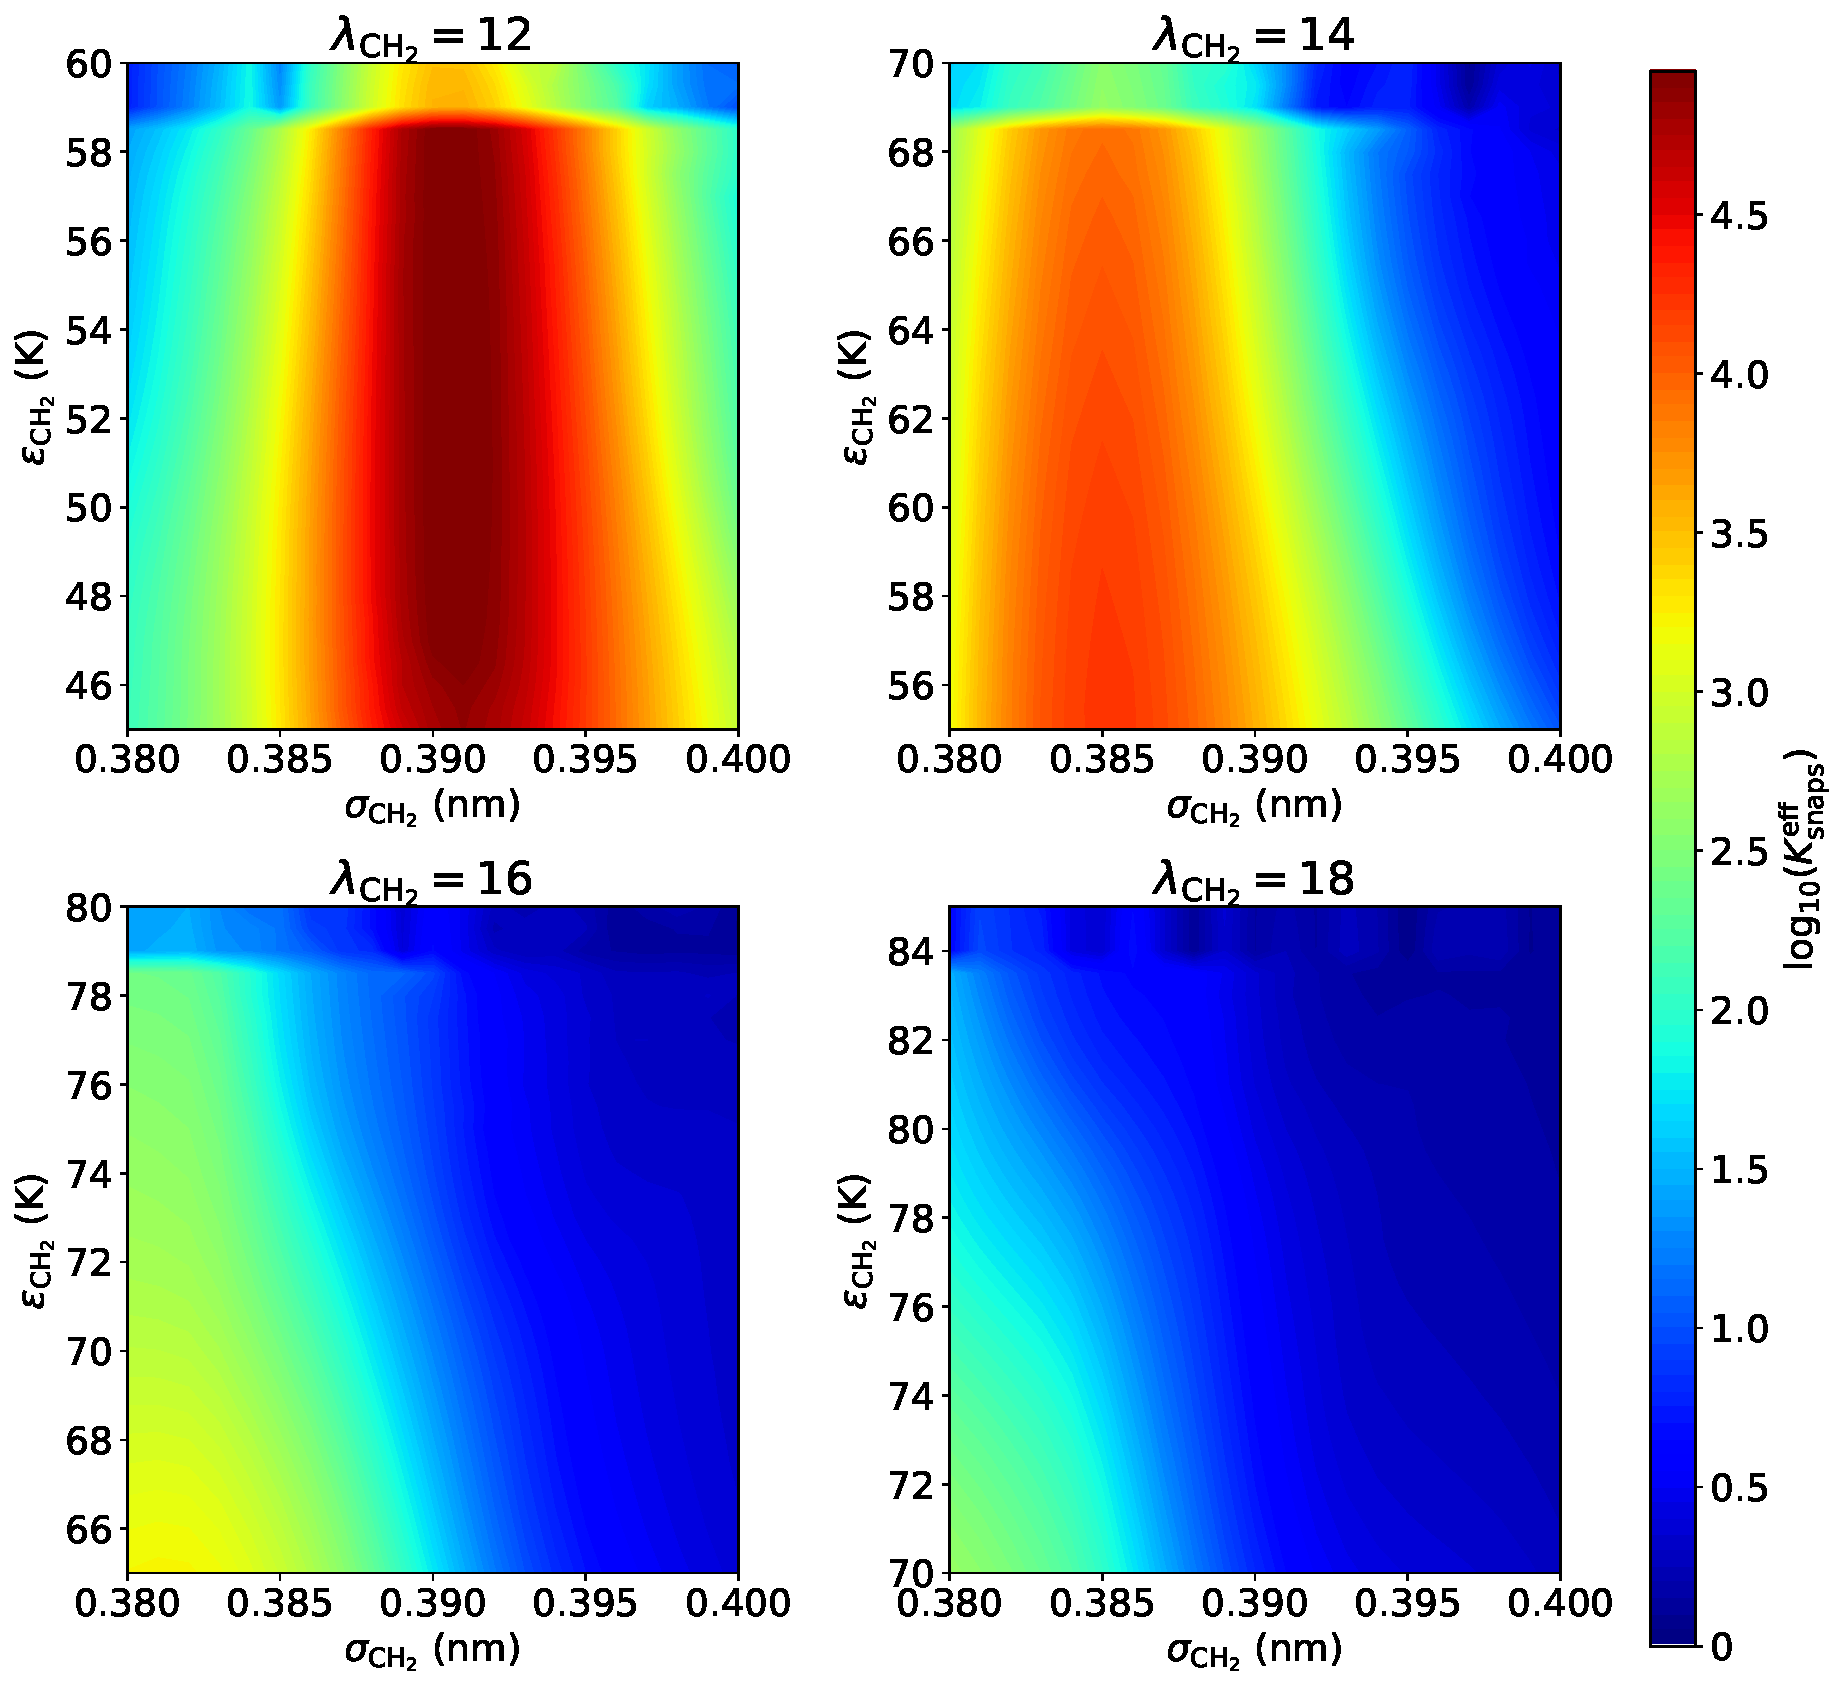
\includegraphics[width=6.4in]{CYC6_Neff_lam.pdf}
		\caption{Average number of effective samples in the liquid phase $(\bar K_{\rm snaps}^{\rm eff, liq})$ with respect to $\epsilon_{\rm CH_2}$ and $\sigma_{\rm CH_2}$ for cyclohexane. $K_{\rm snaps}^{\rm eff, liq} \gg 50$ over a wide range of parameters when $\lambda_{\rm rr} = \lambda_{\rm ref} = 12$ (top-left panel), while $K_{\rm snaps}^{\rm eff, liq}$ is typically less than $50$ for $\lambda_{\rm rr} \neq \lambda_{\rm ref}$ (other panels). Top-left, top-right, bottom-left, and bottom-right panels correspond $\lambda_{\rm CH_2} = 12$, $\lambda_{\rm CH_2} = 14$, $\lambda_{\rm CH_2} = 16$, $\lambda_{\rm CH_2} = 18$, respectively.}
		\label{fig:Neff_CYC6}
	\end{figure}

%\begin{enumerate}
%	\item We validate that MBAR and HR are statistically indistinguishable with sufficient data by re-analyzing the simulation results of Mick et al. and Barhaghi et al. utilizing MBAR
%	%	\begin{enumerate}
%	%		\item Evaluate all of the compounds that Mohammad has U and N values for (branched alkanes and alkynes) and which have good experimental data
%	%		\item Compare MBAR results with either Potoff's or my own HR results (might be better to use my own for self consistency)
%	%	\end{enumerate}
%	%    \item Validation of the basis function approach
%	\item Epsilon scaling for all the compounds that Mohammad has U and N values for (branched alkanes and alkynes) and which have good experimental data
%	\item We estimate MiPPE generalized and NERD VLE from TraPPE simulations, MiPPE S/L from MiPPE generalized, and TraPPE from MiPPE generalized
%	\item For $\lambda_{\rm ref} = 12$ and $\lambda_{\rm rr} = 16$, MBAR-GCMC predicts vapor density, vapor pressure, and heat of vaporization more accurately than liquid density
%	\item For $\lambda_{\rm ref} = 12$ and $\lambda_{\rm rr} = 12$, i.e., computing NERD from TraPPE simulations, MBAR-GCMC predicts all four properties accurately    
%	\item We present how basis functions allow for rapid computation of wide range of parameter sets:
%	\begin{enumerate}
%%		\item \textit{n}-hexane
%		\item 2-methylpropane
%		\item 2,2-dimethylpropane
%		\item cyclopentane or cyclohexane
%	\end{enumerate}
%	\item We provide supporting information with basis functions for several branched alkanes with TraPPE and MiPPE force fields
%\end{enumerate}
%
%\subsection{Figures}
%
%
%\begin{enumerate}
%	\item Percent deviation between MBAR and HR results for rholiq, rhovap, Psat, and DeltaHv
%	\item Comparison between MBAR bootstrapping and analytical uncertainties and HR uncertainties (?)
%	\item Scaling of epsilon post-simulation for branched alkanes and alkynes
%	\item Prediction of VLE for $\lambda_{\rm ref} \neq \lambda_{\rm rr}$
%	\item Prediction of VLE for $\lambda_{\rm ref} = \lambda_{\rm rr}$
%%	\item Two-D scans of scoring functions for $\epsilon-\sigma$ of CH3 (a) and CH2 (b) for \textit{n}-hexane
%	\item Two-D scans of scoring functions for $\epsilon-\sigma$ of CH3 (a) and CH (b) for 2-methylpropane
%	\item Two-D scans of scoring functions for $\epsilon-\sigma$ of CH3 (a) and C (b) for 2,2-dimethylpropane
%	\item Two-D scans of scoring functions for $\epsilon-\sigma$ of CH2 for cyclopentane or cyclohexane (reference is TraPPE)
%\end{enumerate}

\section{Discussion/Limitations/Future work} \label{sec: Discussion}

As molecular insertion moves are frequently rejected in high density systems, GCMC simulations are typically not reliable at low saturation temperatures $(T_{\rm } < 0.65)$. As ITIC does not suffer from this low-temperature limitation, we recommend combining the MBAR-ITIC and GCMC-MBAR methods when predicting vapor-liquid coexistence properties from near-triple-point to near-critical-point conditions.

The results presented in this study were obtained by performing simulations with only a single reference force field. As shown in previous studies, a logical approach for improving the performance of MBAR is to include additional reference force fields \cite{Postdoc_1,Postdoc_2}. For example, we could include a reference parameter set for each value of $\lambda_{\rm CH_2}$ to increase $K_{\rm snaps}^{\rm eff, liq}$ and, thereby, improve the reliability of liquid phase property estimates.

Although GCMC-HR is a standard approach for computing vapor-liquid coexistence, HR can also been applied to GEMC simulations (GEMC-HR) \cite{Boulougouris2010}. Therefore, while the present study presents how MBAR can be applied to GCMC simulations, an analogous GEMC-MBAR approach is worth investigating in future work.

%
%\begin{enumerate}
%	\item We recommend that future GCMC-VLE studies report the snapshots of $N$ and $U$ and/or basis functions to recompute $U$ as this allows for future force field optimization
%	\item Improvements are possible with multiple $\theta$ or simulating a range of $\mu$ values
%\end{enumerate}

\section{Conclusions} \label{sec: Conclusions}

This study demonstrates how the Multistate Bennett Acceptance Ratio can replace the traditional histogram reweighting approach for estimating vapor-liquid coexistence properties from Grand Canonical Monte Carlo simulations. MBAR and HR are mathematically equivalent in the limit of infinitesimal bin widths when the coexistence properties are computed for a single force field. However, the primary benefit of MBAR is the ability to estimate properties for multiple force fields. This enables rapid non-bonded parameterization without requiring large amounts of simulation. We demonstrate this capability by performing a one-dimensional $\epsilon$-scaling optimization of several branched alkanes and alkynes. We then show how GCMC-MBAR can re-optimize a Lennard-Jones 12-6 potential into a family of Mie $\lambda$-6 potentials for cyclohexane. 

\section{Acknowledgments}

We would like to acknowledge Dr. J. Richard Elliott for his invaluable insights. We are also appreciative of the internal review provided by Eugene Paulechka, Andrei F. Kazakov, Daniel G. Friend, and Marcia L. Huber of the National Institute of Standards and Technology (NIST).

This research was performed while Richard A. Messerly held a National Research Council (NRC) Postdoctoral Research Associateship at NIST and while Michelle C. Anderson held a Summer Undergraduate Research Fellowship (SURF) position at NIST. 

Commercial equipment, instruments, or materials are identified only in order to adequately specify certain procedures. In no case does such identification imply recommendation or endorsement by NIST, nor does it imply that the products identified are necessarily the best available for the intended purpose.

Contribution of NIST, an agency of the United States government; not subject to copyright in the United States.

\bibliography{JCED_FOMMS_references}

%\section{Supporting Information}
%
%\subsection{MBAR VLE estimates}
%
%Provide tables of MBAR estimates
%
%\subsection{Basis functions}
%
%\begin{enumerate}
%	\item Validation that basis functions give accurate energies
%\end{enumerate}
%
%\subsection{Raw data}
%
%\begin{enumerate}
%	\item Comparison of 2-D histograms for TraPPE and MiPPE. MBAR overlap, possible? Probably not without rerunning the simulations.
%\end{enumerate}


\end{document}
